% Revision V5 adviser print-layout corrections, evidence preserved, based on the preserved report source and evidence.
% Borrow structure/academic typesetting only, not any other team's content, names or results.
% Do not overwrite templates/original, frozen experiment outputs or historical research notes.
\documentclass[a4paper,12pt,oneside]{report}
\usepackage{fontspec}
% NetFlow sample: Vietnamese Roman serif (VNR12).
% Liberation Serif is a Unicode Times-compatible alternative, preserving
% Vietnamese diacritics; use system-installed fonts only.
\IfFontExistsTF{Liberation Serif}{\setmainfont{Liberation Serif}}{\setmainfont{TeX Gyre Termes}}
\usepackage[vietnamese]{babel}
\usepackage[a4paper,top=23mm,bottom=23mm,left=30mm,right=23mm,headheight=17pt,headsep=8mm,footskip=11mm]{geometry}
\usepackage{xcolor}
\definecolor{researchred}{RGB}{150,0,23}
\usepackage{amsmath,amssymb,graphicx,array,booktabs,longtable,tabularx}
\usepackage{siunitx}
\sisetup{detect-all,output-decimal-marker={.},group-separator={\,},group-minimum-digits=4,group-digits=integer}
\usepackage{pdflscape}
\usepackage{placeins}
\usepackage{tikz}
\usetikzlibrary{calc}
\usepackage{caption}
\usepackage{float} % keep revision-specific evidence tables beside explanations
\usepackage{fancyhdr}
\usepackage{titlesec}
\usepackage{tocloft}
\usepackage{setspace}
\usepackage{xurl}
\usepackage[unicode,colorlinks=true,linkcolor=researchred,citecolor=researchred,urlcolor=researchred]{hyperref}
\emergencystretch=5em
\setstretch{1.22}
\setlength{\parindent}{15pt}
\setlength{\parskip}{5pt}
\setcounter{secnumdepth}{2}
\setcounter{tocdepth}{2}

% Neutral body and section hierarchy; carmine accent from original PTIT template.
\titleformat{\chapter}[block]{\normalfont\bfseries\centering\fontsize{15}{20}\selectfont\color{black}}{Chương \thechapter.}{0.8em}{\MakeUppercase}
\titleformat{name=\chapter,numberless}[block]{\normalfont\bfseries\centering\fontsize{15}{20}\selectfont\color{black}}{}{0em}{}
\titlespacing*{\chapter}{0pt}{7pt}{16pt}
\titleformat{\section}{\normalfont\bfseries\fontsize{14}{19}\selectfont\color{black}}{\thesection}{0.8em}{}
\titleformat{\subsection}{\normalfont\bfseries\fontsize{12.5}{17}\selectfont\color{black}}{\thesubsection}{0.8em}{}
% Level 3 (e.g. 1.2.1.1) uses a clean unnumbered caption, not another numeral.
\titleformat{\subsubsection}[hang]{\normalfont\bfseries\fontsize{12}{16}\selectfont}{ }{0pt}{}
\titlespacing*{\section}{0pt}{15pt plus 2pt minus 2pt}{7pt}
\titlespacing*{\subsection}{0pt}{10pt plus 2pt minus 1pt}{5pt}
\titlespacing*{\subsubsection}{0pt}{8pt plus 1pt minus 1pt}{3pt}
\usepackage{needspace}
% Avoid stranded headings at page bottoms without forcing unrelated new pages.
\let\originalsection\section
\let\originalsubsection\subsection
\let\originalsubsubsection\subsubsection
\renewcommand{\section}{\needspace{7\baselineskip}\originalsection}
\renewcommand{\subsection}{\needspace{5\baselineskip}\originalsubsection}
\renewcommand{\subsubsection}{\needspace{4\baselineskip}\originalsubsubsection}
\captionsetup{font=small,labelfont={bf,color=black},labelsep=period}
\renewcommand{\cftchappresnum}{Chương~}
\setlength{\cftchapnumwidth}{6em}
\renewcommand{\cftsecleader}{\cftdotfill{\cftdotsep}}
\renewcommand{\cftsubsecleader}{\cftdotfill{\cftdotsep}}
\renewcommand{\cftfigpresnum}{Hình~}
\setlength{\cftfignumwidth}{6em}
\renewcommand{\cfttabpresnum}{Bảng~}
\setlength{\cfttabnumwidth}{6em}
\makeatletter
\let\originalcontentsline\contentsline
\makeatother

% Header/footer aligned with PTIT report; no unverified image/signature.
\pagestyle{fancy}
\fancyhf{}
\fancyhead[L]{\footnotesize\color{black} ĐỀ TÀI NCKH SINH VIÊN}
\fancyhead[R]{\footnotesize\color{black} ENSEMBLE LEARNING -- NIDS}
\fancyfoot[L]{\footnotesize\color{black} Mã đề tài: 09-SV-2026-CNTT2}
\fancyfoot[R]{\footnotesize\color{black} \thepage}
\renewcommand{\headrulewidth}{0.35pt}
\renewcommand{\footrulewidth}{0.35pt}
\fancypagestyle{plain}{\fancyhf{}\fancyhead[L]{\footnotesize\color{black} ĐỀ TÀI NCKH SINH VIÊN}\fancyfoot[L]{\footnotesize\color{black} 09-SV-2026-CNTT2}\fancyfoot[R]{\footnotesize\color{black} \thepage}\renewcommand{\headrulewidth}{0.35pt}\renewcommand{\footrulewidth}{0.35pt}}

\begin{document}
\raggedbottom
\begin{titlepage}
\thispagestyle{empty}
\begin{tikzpicture}[remember picture,overlay]
\draw[black,line width=.55pt] ($(current page.north west)+(2.0cm,-1.45cm)$) rectangle ($(current page.south east)+(-1.75cm,1.45cm)$);
\draw[researchred!70,line width=1.1pt] ($(current page.north west)+(2.18cm,-1.62cm)$) rectangle ($(current page.south east)+(-1.92cm,1.62cm)$);
\end{tikzpicture}
\centering
{\fontsize{12}{16}\selectfont BỘ KHOA HỌC VÀ CÔNG NGHỆ\par}
{\fontsize{13}{17}\selectfont\bfseries HỌC VIỆN CÔNG NGHỆ BƯU CHÍNH VIỄN THÔNG\par}
{\fontsize{13}{17}\selectfont\bfseries CƠ SỞ TẠI TP. HỒ CHÍ MINH\par}
{\fontsize{11}{15}\selectfont Khoa/đơn vị: \textbf{Khoa Công nghệ Thông tin 2}\par}
\vspace{4mm}
{\color{researchred}\rule{0.35\textwidth}{0.6pt}\par}
\vspace{8mm}

\includegraphics[width=25mm]{../templates/original/latex/assets/Logo_PTIT_University.png}
\vspace{7mm}

{\large\bfseries ĐỀ TÀI NGHIÊN CỨU KHOA HỌC SINH VIÊN\par}
\vspace{6mm}
{\normalsize Mã số đề tài: \textbf{09-SV-2026-CNTT2}\par}
\vspace{7mm}
{\color{researchred}\fontsize{18}{23}\selectfont\bfseries NGHIÊN CỨU ENSEMBLE LEARNING\\[3mm] CHO BÀI TOÁN PHÁT HIỆN XÂM NHẬP MẠNG\par}
\vspace{6mm}
{\color{black}\normalsize Thực nghiệm phân loại nhị phân trên UNSW-NB15\par}
\vfill
\begin{minipage}{0.91\linewidth}
\raggedright
\small
\begin{tabular}{@{}p{.28\linewidth}p{.40\linewidth}p{.21\linewidth}@{}}
\textbf{\shortstack[l]{Sinh viên\\thực hiện:}} & Dương Ngọc Phú & N23DCDK055\\[4pt]
& Phạm Thế Vỹ & N23DCCN205\\[4pt]
& Vũ Văn Kiên & N23DCDT029\\[4pt]
& Lê Hoàng Nguyên Quân & N23DCDT042\\[7pt]
\textbf{Lớp:} & \multicolumn{2}{l}{E23CQCE01-N}\\[5pt]
\textbf{\shortstack[l]{Giảng viên\\hướng dẫn:}} & \multicolumn{2}{l}{TS. Lê Ngọc Hiếu}\\
\end{tabular}
\end{minipage}
\vfill
{\normalsize\bfseries TP. Hồ Chí Minh -- 2026\par}
\end{titlepage}

\pagenumbering{roman}
% PTIT-style preliminary pages. Do not reuse identities or statements from sample group.
\chapter*{LỜI CAM ĐOAN}
\addcontentsline{toc}{chapter}{Lời cam đoan}
Nhóm sinh viên thực hiện đề tài gồm Dương Ngọc Phú (N23DCDK055), Phạm Thế Vỹ (N23DCCN205), Vũ Văn Kiên (N23DCDT029) và Lê Hoàng Nguyên Quân (N23DCDT042), thuộc lớp E23CQCE01-N, dưới sự hướng dẫn của TS. Lê Ngọc Hiếu.

Chúng em xác nhận rằng các nội dung mô tả quy trình, dữ liệu và kết quả thực nghiệm trong báo cáo được trình bày nhất quán với dữ liệu, chương trình thực nghiệm và bảng kết quả. Các công trình tham khảo được trích dẫn; các giới hạn về mẫu, thiết kế kiểm định và khả năng tái lập được công khai để người đọc có thể đánh giá phạm vi kết luận.

Nhóm sinh viên chịu trách nhiệm tự kiểm tra tính chính xác và tính nguyên gốc của bản báo cáo trước khi nộp theo quy định của Học viện. Việc ký tên xác nhận do chính các thành viên thực hiện khi hoàn thiện hồ sơ nộp.

\vspace{1.8cm}
\begin{flushright}
TP. Hồ Chí Minh, năm 2026\\[10pt]
Nhóm sinh viên thực hiện
\end{flushright}

\clearpage
\chapter*{LỜI CẢM ƠN}
\addcontentsline{toc}{chapter}{Lời cảm ơn}
Nhóm sinh viên trân trọng cảm ơn giảng viên hướng dẫn TS. Lê Ngọc Hiếu đã đồng hành trong quá trình thực hiện đề tài nghiên cứu khoa học về Ensemble Learning cho phát hiện xâm nhập mạng.

Chúng em cảm ơn các thầy cô của Khoa Công nghệ Thông tin 2, Học viện Công nghệ Bưu chính Viễn thông, vì nền tảng kiến thức và môi trường học thuật hỗ trợ quá trình học tập, nghiên cứu. Báo cáo được thực hiện dựa trên những dữ liệu và nguồn tham khảo có ghi nhận, với mong muốn làm rõ chất lượng thực nghiệm cũng như những hạn chế khi ứng dụng các mô hình học máy cho NIDS.

Nhóm mong nhận được những ý kiến nhận xét và phản biện để tiếp tục hoàn thiện nghiên cứu.

\vspace{1.8cm}
\begin{flushright}
TP. Hồ Chí Minh, năm 2026\\[10pt]
Nhóm sinh viên thực hiện
\end{flushright}

\clearpage
\renewcommand{\contentsname}{MỤC LỤC}
\renewcommand{\listfigurename}{DANH SÁCH HÌNH VẼ}
\renewcommand{\listtablename}{DANH SÁCH BẢNG}
\tableofcontents
\clearpage
% Danh mục từ viết tắt: alphabet theo mã viết tắt (A-Z), giữ thuật ngữ/ý nghĩa khoa học không thay đổi.
\chapter*{DANH MỤC TỪ VIẾT TẮT}
\addcontentsline{toc}{chapter}{Danh mục từ viết tắt}
\begin{longtable}{@{}p{.115\linewidth}p{.345\linewidth}p{.485\linewidth}@{}}
\toprule
\textbf{Ký hiệu} & \textbf{Thuật ngữ đầy đủ} & \textbf{Ý nghĩa trong nghiên cứu}\\
\midrule
\endfirsthead
\toprule
\textbf{Ký hiệu} & \textbf{Thuật ngữ đầy đủ} & \textbf{Ý nghĩa trong nghiên cứu}\\
\midrule
\endhead
AP & Average Precision & Chỉ số tóm tắt quan hệ Precision--Recall theo các ngưỡng dự đoán.\\
CI & Confidence Interval & Khoảng giá trị ước lượng thể hiện bất định của một đại lượng thống kê theo quy trình đã chọn.\\
CV & Cross-Validation & Phương pháp chia tập huấn luyện thành nhiều phần để ước lượng chất lượng khi phát triển mô hình.\\
DT & Decision Tree & Mô hình phân loại dựa trên các nhánh điều kiện đối với giá trị đặc trưng.\\
EDA & Exploratory Data Analysis & Khảo sát phân bố, chất lượng dữ liệu và quan hệ giữa các đặc trưng trước huấn luyện.\\
F1 & F1-score & Trung bình điều hòa của Precision và Recall; phản ánh chất lượng cân bằng giữa hai đại lượng.\\
FN & False Negative & Số mẫu Attack bị nhận nhầm là Normal (tấn công bị bỏ sót).\\
FNR & False Negative Rate & Tỷ lệ Attack bị bỏ sót, tính bằng FN/(FN+TP).\\
FP & False Positive & Số mẫu Normal bị nhận nhầm là Attack (cảnh báo giả).\\
FPR & False Positive Rate & Tỷ lệ Normal bị cảnh báo nhầm, tính bằng FP/(FP+TN).\\
FS & Feature Selection & Quá trình chọn tập đặc trưng đầu vào nhằm cân bằng thông tin dự đoán và chi phí tính toán.\\
IDS & Intrusion Detection System & Hệ thống giám sát và phát hiện hoạt động có dấu hiệu xâm nhập.\\
LR & Logistic Regression & Bộ phân loại ước lượng xác suất thuộc lớp Attack từ các đặc trưng đầu vào.\\
MCC & Matthews Correlation Coefficient & Chỉ số tương quan giữa nhãn thật và dự đoán, sử dụng đủ bốn ô ma trận nhầm lẫn.\\
ML & Machine Learning & Phương pháp học quy luật từ dữ liệu nhằm dự đoán nhãn của lưu lượng mới.\\
NIDS & Network Intrusion Detection System & Hệ thống IDS phân tích dữ liệu lưu lượng mạng để nhận biết hành vi tấn công.\\
OOF & Out-of-Fold & Dự đoán trên phần dữ liệu không dùng để huấn luyện mô hình ở lượt chia fold tương ứng.\\
RF & Random Forest & Bộ phân loại kết hợp nhiều cây quyết định để dự đoán nhãn hoặc xác suất tấn công.\\
SMD & Standardized Mean Difference & Mức chênh lệch trung bình giữa hai nhóm, quy đổi theo độ phân tán của đặc trưng.\\
TN & True Negative & Số mẫu Normal được mô hình dự đoán đúng là Normal.\\
TP & True Positive & Số mẫu Attack được mô hình dự đoán đúng là Attack.\\
\bottomrule
\end{longtable}

\clearpage
\listoffigures
\clearpage
\listoftables
\clearpage

\pagenumbering{arabic}
\chapter{CƠ SỞ LÝ THUYẾT}
\label{chap:ly-thuyet}
\section{Bối cảnh và mục tiêu nghiên cứu}
\label{chap:gioi-thieu}

\subsection{Bối cảnh và động cơ}
Hệ thống phát hiện xâm nhập mạng (Network Intrusion Detection System, NIDS) nhằm nhận diện lưu lượng có dấu hiệu tấn công từ các quan sát mạng. Các bộ phân loại học máy có thể phát hiện những mẫu phức tạp trong dữ liệu flow, nhưng điểm số cao trên một benchmark không tự bảo đảm hiệu quả trong các bối cảnh triển khai khác nhau. Cách tạo và làm sạch dữ liệu, lựa chọn đặc trưng, chia tập và các loại sai số có thể ảnh hưởng đáng kể đến diễn giải thí nghiệm.

Ensemble Learning kết hợp dự đoán từ nhiều bộ phân loại. Tổng quan của Tama và Lim nhấn mạnh hai lựa chọn thiết kế: thành phần mô hình cơ sở và phương pháp kết hợp \cite{legacyL01}. Voting, Stacking và lựa chọn đặc trưng đều đã được nghiên cứu trước đây; việc áp dụng riêng các kỹ thuật này không tạo thành đóng góp thuật toán mới \cite{legacyL04,legacyL05,legacyL06,legacyL12}. Vì vậy, giá trị của nghiên cứu phụ thuộc vào giao thức có thể truy vết, cách mô tả đúng các loại lỗi, sự đối chiếu chi phí và diễn giải thận trọng độ bất định.

\subsection{Vấn đề nghiên cứu}
Nghiên cứu tập trung vào bài toán nhị phân \textbf{Normal/Attack} của UNSW-NB15. Hai tập TRAIN và TEST chính thức được giữ riêng; các mô hình được lựa chọn trong giai đoạn phát triển trên TRAIN và đánh giá cuối bằng cấu hình đã khóa. Sau đánh giá lịch sử, phần mở rộng P21 được thực hiện trên internal validation của TRAIN với năm seed và năm cấu hình matched; đây là thí nghiệm hậu nghiệm, không truy cập official TEST để tinh chỉnh. Nghiên cứu không xây dựng bộ phân loại đa lớp, cũng chưa kiểm nghiệm trên dữ liệu triển khai độc lập.

Vấn đề trung tâm là liệu các mô hình cơ sở có dạng sai số bổ sung giúp ensemble cải thiện kết quả so với một mô hình đơn mạnh hay chủ yếu làm thay đổi đánh đổi giữa báo động giả (FP) và tấn công bị bỏ sót (FN). Bên cạnh chất lượng dự đoán, nghiên cứu xem xét chi phí huấn luyện, suy luận và lựa chọn đặc trưng. Đây là nghiên cứu trường hợp trên một benchmark, không nhằm chứng minh ưu thế chung của Ensemble Learning.

\subsection{Các vấn đề nghiên cứu}
Để đánh giá chất lượng và giới hạn của các mô hình phát hiện xâm nhập, nghiên cứu tập trung vào năm vấn đề sau:

\begin{description}
\item[RQ1 --- Hiệu quả Ensemble:] Liệu ensemble có cải thiện \emph{ổn định} so với mô hình học máy đơn trong một protocol đánh giá tương ứng? Phần lịch sử không đo độ ổn định qua nhiều lần huấn luyện; phần P21 bổ sung năm FIT seed trên cùng một internal validation, chưa phải external confirmation.
\item[RQ2 --- Đặc trưng và chi phí:] Hai cấu hình với số lượng đặc trưng khác nhau thể hiện ra sao về hiệu năng và chi phí? Phân tích cuối chưa tách được tác động riêng của số đặc trưng.
\item[RQ3 --- Sai số bổ sung:] Mức hiệu năng quan sát có liên hệ thế nào với sự khác nhau giữa sai số của các mô hình cơ sở? Bằng chứng hiện có mang tính mô tả, chưa xác lập quan hệ nhân quả.
\item[RQ4 --- Độ nhạy với overlap:] Chất lượng và thứ hạng mô hình thay đổi thế nào khi chỉ xét các mẫu TEST không trùng vector với TRAIN?
\item[RQ5 --- Mất cân bằng lớp:] Các phương án xử lý mất cân bằng liên hệ thế nào với Recall, Macro-F1 và số Attack bị bỏ sót?
\end{description}

Năm vấn đề trên được phân tích bằng giao thức thực nghiệm ở Chương~\ref{chap:phuong-phap} và các kết quả ở Chương~\ref{chap:ket-qua-thao-luan}.

\subsection{Mục tiêu và đóng góp nghiên cứu}
Nghiên cứu đóng góp một đối chiếu thực nghiệm giữa Random Forest, Voting và Stacking trên split chính thức; khảo sát dự đoán ngoài fold và độ đa dạng sai số trong giai đoạn phát triển; so sánh hai pipeline theo hiệu năng và chi phí; đồng thời trình bày Macro-F1, MCC, FPR, FNR, hiệu số theo cặp và lỗi theo họ Attack trong phạm vi bài toán nhị phân.

Những kết quả này có giá trị thực nghiệm trong phạm vi một nghiên cứu trường hợp, nhưng chưa đủ cơ sở để khẳng định thuật toán Ensemble Learning mới, ưu thế tổng thể của Stacking hay khả năng khái quát ngoài UNSW-NB15. Phần đối chiếu với công trình trước được giới hạn ở các nguồn đã kiểm tra phương pháp; đây không phải tổng quan hệ thống đầy đủ của lĩnh vực.

\subsection{Bố cục báo cáo}
Chương~\ref{chap:ly-thuyet} trình bày cơ sở lý thuyết và các hướng nghiên cứu liên quan. Chương~\ref{chap:dataset-eda} giới thiệu dữ liệu và quy trình tiền xử lý. Chương~\ref{chap:phuong-phap} mô tả mô hình và cách thực hiện thí nghiệm. Chương~\ref{chap:ket-qua-thao-luan} phân tích kết quả huấn luyện và kiểm thử. Chương~\ref{chap:ban-luan} thảo luận về ý nghĩa, hạn chế và hướng phát triển của nghiên cứu.

\section{Các thuật toán học máy và phương pháp kết hợp}


\subsection{Phát hiện xâm nhập dựa trên đặc trưng luồng mạng}
Hệ thống phát hiện xâm nhập mạng (NIDS) phân tích các quan sát về lưu lượng để phân biệt hoạt động bình thường và hoạt động có dấu hiệu tấn công. Một flow có thể được mô tả bằng giao thức, trạng thái kết nối, số gói, lượng byte, thời lượng, thông lượng và các thống kê thời gian. Những biến này làm dữ liệu có thể biểu diễn bằng bảng để áp dụng học máy, nhưng không chứa mọi thông tin của payload hoặc ngữ cảnh vận hành.

Trong báo cáo này, đơn vị dự đoán là một \emph{dòng dữ liệu UNSW-NB15}. Mỗi dòng gồm vector $x=(x_1,\ldots,x_p)$ và nhãn $y\in\{0,1\}$, trong đó $0$ là Normal và $1$ là Attack. Đây chưa phải một quyết định theo session hay một xác nhận của chuyên gia về sự cố thực tế. Biến \texttt{attack\_cat} được giữ để phân tích lỗi theo nhãn thật sau kiểm thử, chứ không phải mục tiêu đã chứng minh của một bộ phân loại đa lớp.

\subsubsection{Quy trình biến đổi và leakage}
Dữ liệu đầu vào có thể có biến số và biến phân loại, cần xử lý thiếu, mã hóa và chuẩn hóa tương ứng. Một nguyên tắc phương pháp quan trọng là mọi tham số học được từ dữ liệu, như thống kê chuẩn hóa, danh mục encoding hoặc cấu hình Feature Selection, phải được tính từ tập huấn luyện được phép dùng trong từng bước validation rồi áp dụng cho tập còn lại. \texttt{Pipeline} hỗ trợ quản lý chuỗi thao tác nhưng không thể tự loại trừ mọi vấn đề do quan sát quá giống nhau giữa các fold hoặc do chọn feature trước outer CV.

Độc lập ở cấp dòng và độc lập ở cấp phiên là hai giả định khác nhau. Nhiều flow có thể chia sẻ host, thời gian, dịch vụ hoặc cách tạo lưu lượng. Nếu chỉ chia ngẫu nhiên ở cấp dòng, điểm test hoặc validation có thể cao do hai phần chứa những mẫu tương tự. Ngược lại, việc phát hiện vector trùng cũng không tự chứng minh hai dòng là cùng một phiên. Do đó nghiên cứu kiểm tra overlap theo định nghĩa rõ ràng và giữ nguyên giới hạn về nguồn gốc traffic.

\subsubsection{Sai số của bộ phát hiện}
False positive (FP) là Normal bị báo Attack, làm tăng công việc xác minh cảnh báo; false negative (FN) là Attack bị trả về Normal, có thể làm bỏ sót sự kiện cần chú ý. Giá trị chi phí của FP/FN tùy môi trường triển khai và chưa được đo trong đề tài, nên không thể giả định một lỗi bỏ sót có giá trị đúng bằng một báo động giả. Việc đọc riêng FPR và FNR giúp trình bày đánh đổi này minh bạch hơn một chỉ số Accuracy duy nhất.

\subsection{Mô hình Logistic Regression}
Logistic Regression là mô hình tuyến tính xác suất. Đối với phân loại nhị phân, giá trị dự đoán dương có thể viết:
\begin{equation}
\widehat p(y=1\mid x)=\sigma(w^\top x+b),\qquad \sigma(z)=\frac{1}{1+e^{-z}}.
\label{eq:lr}
\end{equation}
Một ngưỡng biến xác suất thành nhãn; threshold không nhất thiết phải bằng 0,5 trong mọi ứng dụng, nhưng nghiên cứu cuối đã khóa tại 0,5 trước official TEST. Điều chuẩn trong Logistic Regression kiểm soát độ lớn hệ số để hạn chế khớp quá mức. Đối với dữ liệu NIDS có quan hệ phi tuyến phức tạp, một mô hình tuyến tính có thể thiếu năng lực biểu diễn so với các mô hình cây, nhưng tính khác nhau của bề mặt quyết định lại có thể tạo dạng sai số bổ sung trong ensemble.

Trong chuỗi thực nghiệm, Logistic Regression được xem xét ở tầng base và meta. Vai trò này không chứng minh LR riêng lẻ tối ưu; sự hữu ích phải quan sát qua OOF predictions, độ đa dạng lỗi, và hiệu quả cuối trong protocol thống nhất. Nếu chỉ xét tập TEST rồi lựa chọn lại thành viên có chỉ số tốt nhất thì sẽ phá vỡ ranh giới đánh giá đã khóa.

\subsection{Decision Tree và Random Forest}
\subsubsection{Decision Tree}
Decision Tree chia dữ liệu bằng các điều kiện theo biến và ngưỡng. Một thước đo mức hỗn tạp của nút là Gini:
\begin{equation}
G(D)=1-\sum_{k=0}^{1}p_k^2,
\label{eq:gini}
\end{equation}
với $p_k$ là tỷ trọng lớp $k$ tại nút. Cây có thể biểu diễn điều kiện phi tuyến và tương tác giữa các đặc trưng, nhưng cây quá sâu dễ học các chi tiết riêng của TRAIN. Những siêu tham số như độ sâu tối đa, số quan sát tối thiểu ở lá hoặc số đặc trưng được xét tại mỗi lần tách có thể kiểm soát độ phức tạp.

Decision Tree không nhất thiết có độ chính xác tổng thể cao bằng Random Forest. Khi nó được chọn vào Stacking, lý do phương pháp hợp lệ là kiểm tra liệu một mô hình có cấu trúc sai số khác biệt có đóng góp hiệu quả hay không, thay vì giả định mô hình yếu kết hợp với mô hình mạnh luôn làm kết quả tốt hơn.

\subsubsection{Random Forest}
Random Forest kết hợp nhiều cây được fit với tính ngẫu nhiên trong lấy mẫu và lựa chọn feature. Một mô tả của xác suất dự đoán là:
\begin{equation}
\widehat p_{\mathrm{RF}}(x)=\frac{1}{T}\sum_{t=1}^{T}\widehat p_t(y=1\mid x).
\label{eq:rf}
\end{equation}
Tăng số cây thường đòi hỏi thêm thời gian train, suy luận và bộ nhớ. Tuy vậy, sự thay đổi hiệu năng không tuyến tính theo số cây, và việc tăng mô hình không bảo đảm vượt một mô hình ít cây hơn trên dữ liệu cụ thể. Trong cấu hình cuối RF-42 có 300 cây, còn RF-17 có 150 cây, kích thước lá cũng khác; mọi kết luận về riêng Feature Selection phải tránh so sánh này như một đối chứng chỉ thay số feature.

\subsection{Voting, Stacking và sai số bổ sung}
\subsubsection{Hard voting và weighted soft voting}
Hard voting chọn nhãn theo số thành viên bình chọn \cite{legacyL01,legacyL05}. Weighted soft voting tổng hợp xác suất từ các model:
\begin{equation}
\widehat p_{\mathrm{vote}}(x)=\sum_{m=1}^{M}w_m\widehat p_m(x),\quad
w_m\ge 0,\quad\sum_{m=1}^{M}w_m=1.
\label{eq:voting}
\end{equation}
Trọng số dựa vào một tập validation riêng có thể điều chỉnh ưu tiên thành viên, nhưng chỉ số chất lượng cá nhân không nhất thiết dự báo đóng góp trong ensemble. Nếu tất cả base learners sai trên các dòng giống nhau, lấy trung bình dự đoán không có cơ chế sửa những lỗi chung ấy. Do đó diversity là biến quan sát có ý nghĩa, chứ không phải bằng chứng bắt buộc cho superiority.

\subsubsection{Out-of-fold training của Stacking}
Stacking sử dụng một meta learner để học ánh xạ từ dự đoán của các base learners sang kết quả cuối \cite{legacyL06}. Nếu dùng dự đoán trên chính tập fit của base learners để train meta, tầng meta có thể nhận đầu vào quá lạc quan. Out-of-fold (OOF) giảm vấn đề này: ở mỗi fold, base learner chỉ fit trên các fold khác và tạo xác suất cho fold hiện hành. Ghép lại cho mỗi dòng huấn luyện một dự đoán chưa được base learner fit trực tiếp trên dòng đó:
\begin{equation}
Z_{i,m}=\widehat p_m^{(-k(i))}(x_i),\qquad
\widehat p_{\mathrm{stack}}(x)=g\left(\widehat p_1(x),\ldots,\widehat p_M(x)\right).
\label{eq:stack}
\end{equation}
Mô hình meta trong Stacking-42 là Logistic Regression. Trong suy luận cuối, các base learners được refit trên TRAIN được phép rồi đưa xác suất mới qua meta learner. Tuy nhiên, một Stacking dùng OOF không có nghĩa mọi bước chọn feature, tuning meta và lựa chọn mô hình đã được đưa vào nested CV hoàn toàn. Trong nghiên cứu này, meta tuning chưa fully nested và tập stable features được chọn trên official TRAIN trước development CV.

\begin{figure}[htbp]
\centering
\fcolorbox{researchred!40}{white}{\begin{minipage}{0.9\linewidth}\centering
\textbf{Official TRAIN: phát triển mô hình}\\[3mm]
$\downarrow$\\[1mm]
K-fold OOF: LR \quad DT \quad RF\\[2mm]
$\downarrow$\\[1mm]
Ma trận xác suất OOF $\longrightarrow$ Meta Logistic Regression\\[2mm]
$\downarrow$\\[1mm]
\textbf{Đóng băng candidate và threshold}\\[2mm]
$\downarrow$\\[1mm]
\textcolor{researchred}{\textbf{Official TEST: đánh giá một lần sau freeze}}
\end{minipage}}
\caption{Sơ đồ nguyên lý Stacking/OOF và ranh giới official TEST. Hình chỉ minh họa giao thức, không chứng minh nested validation đầy đủ.}
\label{fig:stacking-protocol}
\end{figure}

\subsubsection{Double-fault, error correlation và oracle}
Double-fault đo tỷ lệ cùng sai của hai bộ phân loại, error correlation mô tả mức liên hệ giữa các biến chỉ báo lỗi, còn oracle giả định có thể chọn đúng đầu ra của một base model bất kỳ trên mỗi mẫu. Oracle là cận mô tả dưới thông tin nhãn thật, không phải thuật toán dự đoán có thể vận hành trực tiếp. Những chỉ số này cho biết các base learners có thể bổ sung nhau ở đâu, nhưng không trả lời việc meta learner có thực sự học được quy tắc kết hợp đúng hay không. Kết quả voting không thuận lợi trong development vẫn phải được giữ lại để tránh thiên lệch chỉ báo cáo phương án tốt.

\subsection{Các chiến lược Feature Selection}
Filter selection sử dụng phép đo thống kê để xếp hạng biến; wrapper selection đánh giá trực tiếp các tập con thông qua mô hình; embedded selection khai thác cơ chế lựa chọn trong khi fit \cite{legacyL08,legacyL12}. Các phương pháp có ưu nhược điểm khác nhau về chi phí, tương tác biến và thiên lệch theo model. Tính ổn định của feature được chọn qua nhiều lần lặp giúp hạn chế phụ thuộc một phép chia cụ thể, nhưng không chứng minh loại bỏ biến ít quan trọng luôn cải thiện generalization.

Một phép đo gần bằng nhau của RF-17 và RF-42 không cho phép suy rằng 25 feature bị bỏ đều vô dụng. Mục tiêu của việc giảm feature trong đề tài là khảo sát một \emph{đánh đổi giữa chất lượng và tài nguyên} của hai pipeline cụ thể. Muốn quy kết quả cho riêng số feature phải giữ cố định mọi thành phần khác của RF và lồng lựa chọn feature trong outer folds.

\subsection{Các chỉ số đánh giá và diễn giải thống kê}
\subsubsection{Precision, Recall, Macro-F1 và MCC}
Với Attack là lớp dương:
\begin{align}
\mathrm{Precision}&=\frac{\mathrm{TP}}{\mathrm{TP}+\mathrm{FP}},&
\mathrm{Recall}&=\frac{\mathrm{TP}}{\mathrm{TP}+\mathrm{FN}},\\
\mathrm{F1}&=\frac{2\mathrm{Precision}\,\mathrm{Recall}}{\mathrm{Precision}+\mathrm{Recall}},&
\mathrm{FPR}&=\frac{\mathrm{FP}}{\mathrm{FP}+\mathrm{TN}},\\
\mathrm{FNR}&=\frac{\mathrm{FN}}{\mathrm{FN}+\mathrm{TP}},&
\mathrm{Detection\ Rate}&=1-\mathrm{FNR}.
\end{align}
Macro-F1 lấy trung bình F1 hai lớp với trọng số bằng nhau. Weighted-F1 lấy trung bình theo support. MCC sử dụng toàn bộ ma trận nhầm lẫn:
\begin{equation}
\mathrm{MCC}=\frac{\mathrm{TP}\mathrm{TN}-\mathrm{FP}\mathrm{FN}}
{\sqrt{(\mathrm{TP}+\mathrm{FP})(\mathrm{TP}+\mathrm{FN})
(\mathrm{TN}+\mathrm{FP})(\mathrm{TN}+\mathrm{FN})}}.
\label{eq:mcc}
\end{equation}
Macro-F1 khác MCC: Macro-F1 tổng hợp riêng chất lượng F1 của mỗi lớp, còn MCC đo tương quan giữa nhãn thật và nhãn dự đoán dựa trên cả bốn ô. Hai thước đo có thể xếp hạng hai mô hình khác nhau.

\subsubsection{Paired bootstrap và McNemar}
Cùng một dòng TEST được dự đoán bởi hai model, do đó sai số của chúng có cấu trúc cặp. Paired bootstrap lấy mẫu lại chỉ số dòng, áp dụng chung cho hai mô hình và tính hiệu số metric trong mỗi lần lặp. CI 95\% từ các lần lặp cho thấy bất định do các dòng benchmark đã quan sát, chứ không phải độ biến thiên giữa các lần train độc lập hoặc khi chuyển sang mạng khác.

McNemar kiểm tra số dòng A đúng/B sai so với A sai/B đúng. Đây là kiểm định trên \emph{paired correctness}, không phải trực tiếp trên độ chênh lệch Macro-F1. Khi có nhiều phép so sánh, điều chỉnh Holm giới hạn rủi ro báo có ý nghĩa do thử nhiều giả thuyết. Các CI và phép kiểm định không sửa được tính phụ thuộc giữa các dòng flow; đó là giới hạn riêng về đơn vị lấy mẫu.

\section{Các công trình nghiên cứu liên quan}
\label{chap:tong-quan}

\subsection{Ensemble Learning trong NIDS}
Tama và Lim khảo sát có hệ thống hướng Ensemble Learning cho Intrusion Detection và đặt trọng tâm vào base classifier, cách kết hợp và tính phụ thuộc của đánh giá theo benchmark \cite{legacyL01}. Kết quả tổng quan này là cơ sở lựa chọn câu hỏi so sánh thực nghiệm, không thể thay bằng nhận định đơn giản rằng kết hợp nhiều classifier chắc chắn làm hiệu năng tăng.

Các cấu hình kết hợp đã được nghiên cứu theo nhiều hướng: soft voting có thành phần tìm cấu hình tự động \cite{legacyL05}, heterogeneous stacking với các base learners và meta learner được mô tả trong phần phương pháp của Thockchom và cộng sự \cite{legacyL06}, và hướng kết hợp lựa chọn đặc trưng với ensemble \cite{legacyL04,legacyL12}. Các nghiên cứu có phương pháp và tập dữ liệu khác nhau không được coi là baseline matched cho official UNSW-NB15 của đề tài. Việc tồn tại những công trình này giới hạn tuyên bố novelty: đóng góp được định vị ở kiểm toán case study, sự minh bạch về loại lỗi, bằng chứng cặp và chi phí, \emph{không} phải tạo ra Stacking hay Feature Selection.

\subsection{Feature Selection, chuẩn hóa và mất cân bằng}
Việc giảm số đặc trưng có thể thay đổi chất lượng và chi phí của pipeline, nhưng phải tách việc chọn feature khỏi khâu đánh giá nếu muốn ước lượng hiệu ứng thật sự của chiến lược lựa chọn. Các nghiên cứu về filter-based Feature Selection trong IDS \cite{legacyL08}, đặc trưng và chuẩn hóa \cite{legacyL11}, cũng như embedded/correlation selection \cite{legacyL12} là những nguồn đặt phạm vi cho câu hỏi RQ2, không phải bằng chứng rằng RF-17 của chúng tôi cải thiện nhờ \emph{chỉ} loại feature.

Đối với dữ liệu mất cân bằng, nghiên cứu DUEN xem xét dynamic ensemble cùng thành phần xử lý phân bố lớp \cite{legacyL07}. Do đề tài hiện không có so sánh matched resampling/no-resampling dưới cùng điều kiện, không thể kết luận các kỹ thuật cân bằng mẫu là vô ích hoặc có hiệu quả nhân quả từ những kết quả được lưu. Đây vẫn là giới hạn của RQ5.

\subsection{Chất lượng dữ liệu và khả năng khái quát}
Engelen và cộng sự phân tích lỗi và quá trình xử lý trong một bộ dữ liệu IDS khác (CICIDS2017) \cite{legacyL02}; bài học phương pháp luận là cần kiểm toán pipeline và chất lượng dữ liệu, \emph{không} chuyển nguyên các lỗi CICIDS2017 sang UNSW-NB15. Cantone và cộng sự nhấn mạnh sự khác biệt giữa đánh giá trong cùng một dataset và đánh giá cross-dataset \cite{legacyL09}. Nghiên cứu của chúng tôi mới có official holdout cùng một phần exact-duplicate-filtered view; đó không phải external validation hoặc phép đo generalization cross-dataset.

Khảo sát về các loại tấn công chưa biết, không điển hình và biến đổi hình thái \cite{legacyL10} gợi ý yêu cầu đọc kết quả tổng thể trong mối liên hệ với các dạng tấn công khác nhau. Nhưng phân tích \texttt{attack\_cat} ở đây là \emph{nhóm nhãn thật của binary detector}, không phải đo khả năng dự đoán nhãn tấn công đa lớp hoặc unknown-attack deployment.

\subsection{Khoảng trống bằng chứng và giới hạn tổng quan}
So sánh ensemble cần xem xét liệu mô hình có cải thiện hay không, mức thay đổi giữa FP và FN, quan hệ giữa diversity và gain, cùng chi phí của cấu hình đã đánh giá. Trong nghiên cứu này, official holdout và các phân tích cặp được trình bày cùng kết quả hậu nghiệm; các thiết kế về repeated-training stability, nested Feature Selection, temporal split, external validation và matched resampling vẫn nằm ngoài phạm vi thí nghiệm hiện có. Đây là những câu hỏi chưa được giải quyết trong nghiên cứu này, không phải nhận định về toàn bộ lĩnh vực.

Các nhận xét tổng quan ở đây dựa trên những bài báo được trích dẫn trong danh mục tài liệu tham khảo; do khác biệt dữ liệu và giao thức, không sử dụng kết quả từ các nghiên cứu đó như đối chứng trực tiếp cho ba mô hình của đề tài.

\subsection{Đối chiếu phương pháp với một số công trình liên quan}
\label{sec:related-work-direct-comparison}

Bảng~\ref{tab:related-methods-revision} đặt protocol và thành phần phương pháp của đề tài cạnh ba công trình mà phần phương pháp đã được đối chiếu trong phạm vi tư liệu hiện có: Thockchom và cộng sự \cite{legacyL06}, Nassreddine và cộng sự \cite{legacyL12}, và Alsaffar và cộng sự \cite{alsaffar2024shielding}. Các nghiên cứu này giúp định vị cách kết hợp Feature Selection và ensemble trong tài liệu liên quan; khác biệt về bộ dữ liệu, cách chia tập và protocol khiến chúng không phải đối chứng trực tiếp về điểm số.

\par\medskip
\begin{center}
\begingroup
\footnotesize
\renewcommand{\arraystretch}{1.12}
\setlength{\tabcolsep}{4pt}
\captionof{table}{Khác biệt về dữ liệu và phương pháp trong một số nghiên cứu liên quan.}
\label{tab:related-methods-revision}
\begin{tabularx}{\linewidth}{p{0.20\linewidth} X X}
\toprule
Công trình & Dữ liệu và thiết kế được báo cáo & Thành phần phương pháp và quan hệ với nghiên cứu này\\
\midrule
Thockchom và cs. (2023) \cite{legacyL06} & Có UNSW-NB15 và mô tả chia ngẫu nhiên 80/20; split không trùng với official holdout ở đây. & Kết hợp Chi-square với GNB/DT/LR và meta-SGD; là tiền lệ về heterogeneous stacking, không phải baseline matched.\\
Nassreddine và cs. (2025) \cite{legacyL12} & Dùng NSL-KDD và CICIDS2017, không sử dụng official UNSW-NB15 TEST của đề tài. & Kết hợp lựa chọn theo tương quan/embedded với LR meta và SMOTE--TOMEK; không đối chiếu trực tiếp điểm số giữa các split.\\
Alsaffar và cs. (2024) \cite{alsaffar2024shielding} & Báo cáo UNSW-NB15 và CICIDS2017, với mô tả gộp partition trước khi chia ngẫu nhiên 80/20. & Kết hợp MI--Boruta với RF/CatBoost/XGBoost và MLP meta; là tiền lệ gần về phương pháp nhưng khác protocol.\\
Nghiên cứu này & Giữ official TRAIN 175\,341 và TEST 82\,332; phân loại nhị phân Normal/Attack. & So sánh RF-17/RF-42 với Stacking-42, có pooled OOF, paired CI, phân tích FP/FN, chi phí và exact-duplicate-filtered sensitivity.\\
\bottomrule
\end{tabularx}
\endgroup
\end{center}

Ba khái niệm đóng góp cần được phân biệt. Nghiên cứu này không đề xuất methodological novelty cho Stacking hay Feature Selection; các thành phần đó đã có tiền lệ trong tài liệu. Đóng góp nghiên cứu ở đây là case study theo split chính thức, còn empirical contribution là cách đối chiếu cùng các pipeline trên các mẫu holdout bằng metric tổng hợp, sai số theo lớp, độ bất định và chi phí đã lưu. Phạm vi này không phải tuyên bố review đầy đủ toàn lĩnh vực, cũng không cho phép xếp hạng các điểm số được tạo ra từ protocol khác nhau.

Các mô tả trong bảng giới hạn ở thông tin phương pháp đã được kiểm tra trong các nguồn nêu trên. Chi tiết chưa xác minh được giữ ở trạng thái chưa xác định, thay vì diễn giải thành khuyết điểm của công trình trước.


\chapter{DỮ LIỆU VÀ QUY TRÌNH TIỀN XỬ LÝ}
\label{chap:dataset-eda}



\section{Nguồn dữ liệu và quy mô bản ghi}
UNSW-NB15 là bộ dữ liệu mô tả lưu lượng mạng dùng trong nghiên cứu phát hiện xâm nhập, được giới thiệu trong công bố của Moustafa và Slay \cite{moustafa2015unsw}. Đề tài sử dụng chính xác hai file phân chia chính thức: 175\,341 dòng TRAIN và 82\,332 dòng TEST. Mục tiêu thực nghiệm được kiểm chứng là phân loại \emph{Normal/Attack}; tên các nhóm tấn công không được sử dụng làm predictor trong mô hình binary.

\begin{table}[htbp]
\centering\small
\renewcommand{\arraystretch}{1.3}
\setlength{\tabcolsep}{9pt}
\caption{Phân bố hai lớp của các tập UNSW-NB15 chính thức.}
\label{tab:dist-normal-attack}
\begin{tabular}{l S[table-format=6.0] S[table-format=6.0] S[table-format=6.0] S[table-format=2.2]}\toprule
Tập & {Normal} & {Attack} & {Tổng} & {Attack (\%)}\\\midrule
TRAIN & 56000 & 119341 & 175341 & 68.06\\
TEST & 37000 & 45332 & 82332 & 55.06\\\bottomrule
\end{tabular}
\end{table}
Sự khác biệt tỷ lệ Attack giữa TRAIN (68,06\%) và TEST (55,06\%) là một quan sát thực tế của dữ liệu chính thức, không phải tỷ lệ do nghiên cứu tự cân bằng lại. Điều này cho thấy tổng Accuracy và Weighted-F1 có thể chịu ảnh hưởng của cách phân bố lớp; đọc Macro-F1, MCC và chỉ số riêng từng lớp sẽ rõ ràng hơn khi so sánh các pipeline.

\begin{figure}[htbp]
\centering
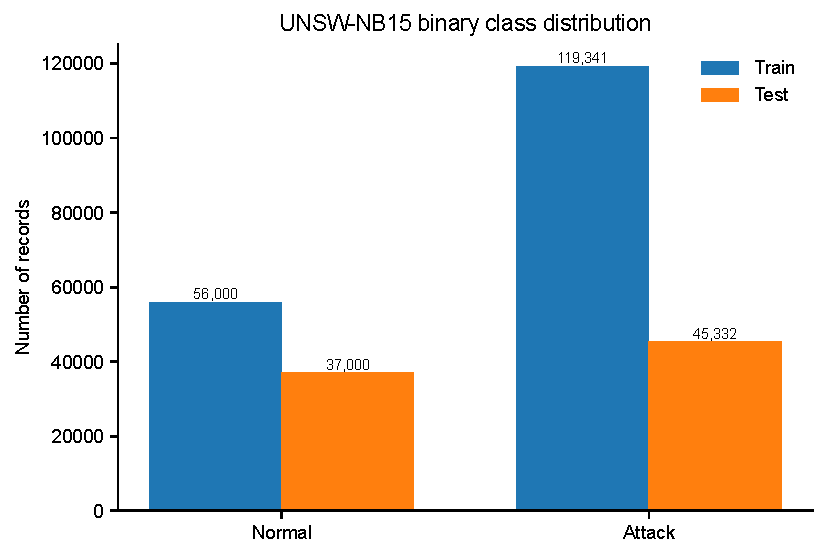
\includegraphics[width=0.86\textwidth]{../results/eda/unsw_nb15/figures/fig01_binary_class_distribution.pdf}
\caption{Phân bố nhãn Normal/Attack trong official TRAIN và TEST, biểu đồ phân bố lớp từ kết quả khảo sát dữ liệu.}
\label{fig:eda-binary}
\end{figure}

\section{Các nhóm tấn công và mức độ chênh lệch}
Ngoài lớp Normal, trường \texttt{attack\_cat} chứa các họ tấn công như Analysis, Backdoor, DoS, Exploits, Fuzzers, Generic, Reconnaissance, Shellcode và Worms. Tại official TEST, Generic chiếm 18\,871 dòng, Exploits 11\,132 dòng và Fuzzers 6\,062 dòng, trong khi Worms chỉ có 44 dòng. Quy mô hỗ trợ không đồng đều có thể làm độ chính xác theo từng nhóm biến động mạnh; một số đếm FN cần được đọc cùng mẫu số của chính nhóm Attack tương ứng.

\begin{figure}[htbp]
\centering
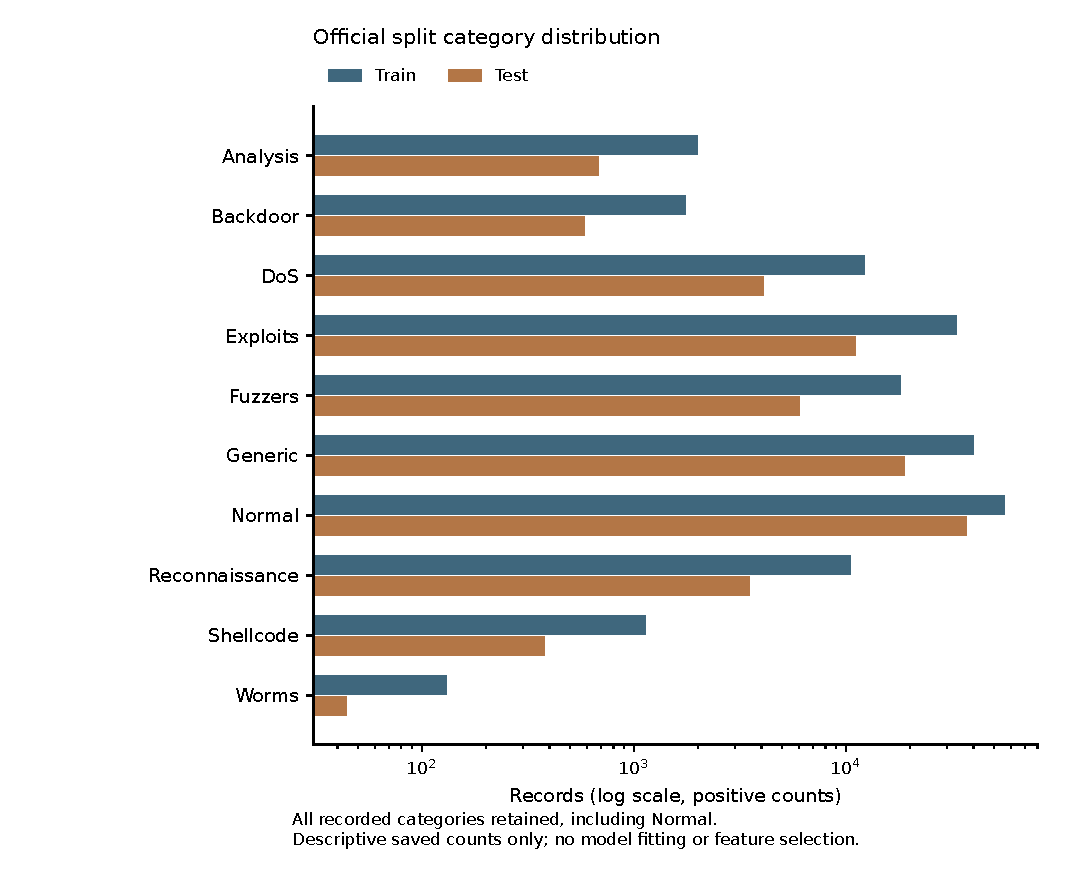
\includegraphics[width=0.94\textwidth]{../results/figures/p16_standalone_2026_10_17_03/category_distribution.pdf}
\caption{Số lượng bản ghi theo \texttt{attack\_cat} của hai tập. Trong nghiên cứu hiện tại, đây là phân tích nhãn thật chứ không phải kết quả một mô hình multiclass.}
\label{fig:eda-attackcats}
\end{figure}

Nhóm Attack ít mẫu không thể được coi là đã phát hiện tốt chỉ vì Accuracy nhị phân tổng thể cao. Một lớp hiếm có thể chỉ góp ít FN vào tổng nhưng lại có FNR cao trong chính lớp đó. Bởi vậy bước Error Analysis trong báo cáo phân nhóm các Attack thật, đồng thời tránh biến các khác biệt nhỏ thành khẳng định về toàn bộ dạng tấn công trong tự nhiên.

\section{Khảo sát thống kê các đặc trưng}
EDA của TRAIN đã kiểm tra 39 biến số. Các tiêu chí thống kê dùng để khám phá không đồng nghĩa phép thử nhân quả. Chẳng hạn, standardized mean difference (SMD) giữa Normal và Attack lớn cho thấy trung bình hai nhóm có khác biệt tương đối theo độ phân tán, nhưng không có nghĩa một feature đơn lẻ là dấu hiệu tấn công đáng tin cậy trong mọi tổ hợp.

Các giá trị SMD lớn về độ lớn trong bảng EDA gồm \texttt{sttl} (1,9430), \texttt{ct\_state\_ttl} (1,3973), \texttt{ct\_dst\_sport\_ltm} (0,9340), \texttt{rate} (0,8692), \texttt{ct\_src\_dport\_ltm} (0,7853), cùng các biến có SMD âm như \texttt{swin} (-0,7636) và \texttt{dload} (-0,7346). Dấu và độ lớn của SMD phản ánh cách định nghĩa hai nhóm trong tập TRAIN; nó không thiết lập hướng tác động của feature lên xác suất bị tấn công.

\begin{figure}[htbp]
\centering
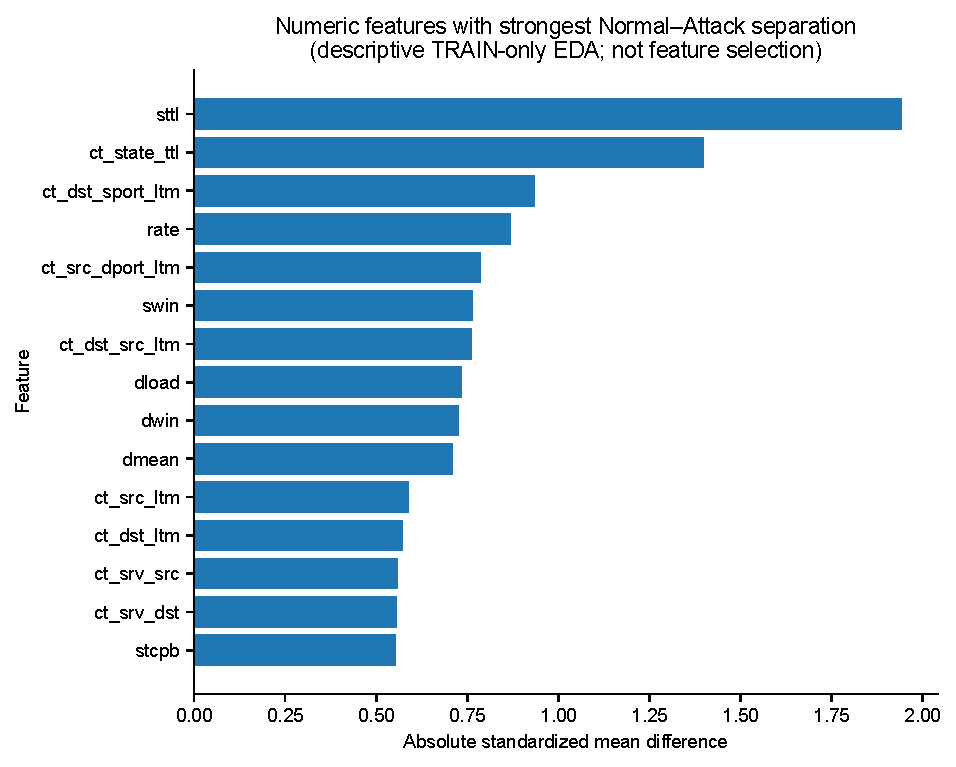
\includegraphics[width=0.96\textwidth]{../results/eda/unsw_nb15/figures/fig03_numeric_class_separation.pdf}
\caption{Khảo sát mức tách biệt Normal/Attack ở một số feature số trên tập huấn luyện. Không dùng biểu đồ này để suy ra quan hệ nhân quả.}
\label{fig:eda-separation}
\end{figure}

\section{Tương quan giữa các đặc trưng}
Trên tập huấn luyện, có 59 cặp feature số đạt $|\rho_{\mathrm{Spearman}}|\geq0,9$. Ví dụ, cặp \texttt{is\_ftp\_login} và \texttt{ct\_ftp\_cmd} có $\rho=1,0000$; \texttt{trans\_depth} và \texttt{ct\_flw\_http\_mthd} có $\rho\approx0,9996$; \texttt{tcprtt} và \texttt{synack} có $\rho\approx0,9968$. Các cặp liên hệ mạnh có thể chứa thông tin trùng lắp trong tập mẫu, nhưng một hệ số tương quan đơn lẻ không cho biết mô hình cây sẽ phụ thuộc vào cặp đó tới mức nào.

\begin{table}[htbp]
\centering
\small
\renewcommand{\arraystretch}{1.25}
\setlength{\tabcolsep}{8pt}
\caption{Năm cặp biến số có tương quan Spearman tuyệt đối lớn nhất trong TRAIN.}
\label{tab:eda-high-correlation}
\begin{tabularx}{\linewidth}{X X S[table-format=1.4]}
\toprule
Biến thứ nhất & Biến thứ hai & {$\rho_{\mathrm{Spearman}}$}\\
\midrule
\texttt{is\_ftp\_login} & \texttt{ct\_ftp\_cmd} & 1.0000\\
\texttt{trans\_depth} & \texttt{ct\_flw\_http\_mthd} & 0.9996\\
\texttt{tcprtt} & \texttt{synack} & 0.9968\\
\texttt{tcprtt} & \texttt{ackdat} & 0.9937\\
\texttt{swin} & \texttt{dwin} & 0.9902\\
\bottomrule
\end{tabularx}
\end{table}

Đối với bước lựa chọn đặc trưng, danh sách cặp tương quan có thể là một nguồn để đề xuất các biến ứng viên, nhưng lựa chọn chính thức còn kết hợp kết quả từ phương pháp filter, embedded và wrapper. Phần EDA được giữ tách khỏi quyết định lựa chọn trên validation; official TEST không được dùng để xếp hạng biến.

\section{Kiểm toán overlap và các view đánh giá}
Quy trình audit kiểm tra vector của 42 feature đã sử dụng cho phân loại nhị phân. Có 8\,541 dòng official TEST trùng vector với ít nhất một dòng official TRAIN; phần còn lại gồm 73\,791 dòng được đặt tên \emph{exact-duplicate-filtered view}. Thuật ngữ \emph{exact-duplicate-filtered view} ở đây chỉ phép loại các dòng TEST có \emph{vector của toàn bộ 42 predictor trùng chính xác} với TRAIN, không hàm ý hai bản ghi cùng session/IP/thời điểm hay có cùng nhãn nguồn; \textbf{không loại bỏ temporal/session leakage}. Số 8\,541 là \emph{số dòng TEST}, không nhất thiết là số vector riêng biệt hay số session bị giao cắt. Các lớp có thể có giá trị feature giống nhau vì cách lượng hóa và tiền xử lý; vì vậy không được tuyên bố mọi trường hợp trùng vector đều là leakage cùng phiên.

\begin{table}[htbp]
\centering\small
\renewcommand{\arraystretch}{1.3}
\setlength{\tabcolsep}{8pt}
\caption{Hai góc nhìn đánh giá cùng thuộc official TEST đã lưu.}
\label{tab:views-test}
\begin{tabularx}{\linewidth}{p{0.24\linewidth} S[table-format=5.0] X}\toprule
View & {Số dòng} & Diễn giải hợp lệ\\\midrule
Official TEST & 82332 & Holdout chính thức dùng cho đánh giá cuối.\\
Exact-duplicate-filtered view & 73791 & TEST sau khi loại dòng có vector 42 đặc trưng trùng với ít nhất một vector TRAIN.\\
Overlap rows & 8541 & Dòng TEST có vector trùng; không đồng nhất với cùng session.\\\bottomrule
\end{tabularx}
\end{table}

Exact-duplicate-filtered view chỉ là một phép phân tích độ nhạy trong cùng bộ dữ liệu, không bảo đảm độc lập theo thời gian hoặc nguồn traffic. Do đó báo cáo trình bày riêng metric official và metric exact-duplicate-filtered, không thay official holdout bằng phần TEST được chọn sau khi quan sát kết quả. Một nghiên cứu đánh giá khả năng khái quát tốt hơn cần một benchmark ngoài hoặc group/temporal split được thiết kế trước, với định nghĩa đơn vị độc lập và quy trình pre-processing nhất quán.

\section{Kết luận về đặc trưng của benchmark}
UNSW-NB15 hỗ trợ một case study IDS nhị phân có quy mô vừa đủ cho đối chiếu nhiều pipeline và có nhãn Attack để phân tích sai số. Tuy nhiên, các chênh lệch lớp, tương quan feature mạnh, sự tồn tại của vector trùng và khả năng phụ thuộc giữa các dòng flow giới hạn phạm vi khái quát. Vì thế hiệu năng trên chính benchmark này được diễn giải dưới các điều kiện của phép đo, không tự chuyển thành khả năng phát hiện xâm nhập trên mạng triển khai thực tế.


\chapter{XÂY DỰNG MÔ HÌNH VÀ THIẾT KẾ THỰC NGHIỆM}
\label{chap:phuong-phap}
\section{Thiết kế nghiên cứu và dữ liệu}
\label{sec:method-design}

Nghiên cứu khảo sát các pipeline học máy và Ensemble Learning cho phát hiện xâm nhập nhị phân trên UNSW-NB15 \cite{moustafa2015unsw}. Nhãn Normal được mã hóa 0 và Attack là 1. Hai partition chính thức được giữ nguyên: TRAIN gồm 175\,341 dòng (56\,000 Normal; 119\,341 Attack), TEST gồm 82\,332 dòng (37\,000 Normal; 45\,332 Attack). Các trường \texttt{id}, \texttt{label} và \texttt{attack\_cat} không thuộc tập predictor. Trường \texttt{attack\_cat} chỉ được dùng sau dự đoán để mô tả các mẫu Attack bị bỏ sót; vì thế kết quả theo họ tấn công không phải phân loại đa lớp.

Thiết kế hướng tới so sánh một baseline Random Forest với Stacking, một cấu hình Random Forest có ít đặc trưng hơn, đồng thời khảo sát lỗi, độ bất định và chi phí quan sát được. Mục tiêu không phải đề xuất thuật toán ensemble mới. Exact-duplicate-filtered view được định nghĩa bằng việc loại khỏi TEST những dòng có vector 42 đặc trưng trùng với vector TRAIN; đây là phân tích độ nhạy trong cùng benchmark, không phải một split độc lập mới.

\section{Lựa chọn đặc trưng và tiền xử lý}
\label{sec:method-feature-selection}

Track 42 giữ toàn bộ đặc trưng dự báo sau khi loại các trường không dùng làm predictor. Track stable17 được xác định trên TRAIN bằng ba nhóm phương pháp filter, L1 và ExtraTrees. Với năm seed \texttt{11, 23, 42, 71, 101}, một biến được xem là ổn định trong từng phương pháp nếu xuất hiện ở ít nhất ba trên năm lượt; tập cuối giữ các biến đáp ứng ngưỡng ở tối thiểu hai phương pháp. Quy tắc này mô tả độ lặp lại của lựa chọn biến trong các lượt đã chạy, không phải bằng chứng về độ ổn định của hiệu năng dự đoán.

Thứ tự 17 biến được khóa là:
\begin{quote}\small\raggedright
\texttt{ct\_srv\_dst}, \texttt{ct\_state\_ttl}, \texttt{dload}, \texttt{dttl},
\texttt{proto}, \texttt{state}, \texttt{sttl}, \texttt{ct\_dst\_ltm},
\texttt{dmean}, \texttt{dwin}, \texttt{is\_sm\_ips\_ports},
\texttt{rate}, \texttt{service}, \texttt{swin},
\texttt{ct\_dst\_sport\_ltm}, \texttt{ct\_dst\_src\_ltm}, \texttt{dbytes}.
\end{quote}
Kết quả RFECV 13 biến là một track riêng, không thay cho stable17. Các biến phân loại \texttt{proto}, \texttt{service} và \texttt{state} được one-hot encode với \texttt{handle\_unknown=ignore}; biến số được chuẩn hóa trong pipeline Logistic Regression, còn Random Forest và Decision Tree dùng phép tiền xử lý phù hợp với estimator. Các phép biến đổi có tham số học được đặt trong pipeline để fit trên phần huấn luyện tương ứng.

Danh sách stable17 được tạo từ toàn bộ official TRAIN trước development cross-validation. Vì vậy, nhãn của các fold validation đã góp phần vào bước chọn biến và điểm development có thể lạc quan so với quy trình nested hoàn toàn. Nhóm coi đây là \textbf{selection bias thật của quy trình lịch sử} cần công khai, không thể sửa hồi tố bằng P21; các kết quả OOF track 42 đặc trưng tại Bảng~\ref{tab:rev-dev} phải phân biệt với đánh giá sử dụng track stable17 lịch sử. TEST không tham gia lựa chọn biến; tuy nhiên, sự phân biệt này không loại bỏ nguy cơ selection optimism trong cross-validation.

\section{Cấu trúc các pipeline}
\label{sec:method-pipelines}

Random Forest huấn luyện nhiều cây quyết định trên các mẫu bootstrap và tập đặc trưng ngẫu nhiên, sau đó tổng hợp xác suất hoặc phiếu dự đoán của các cây. Cấu hình RF-42 có 300 cây, \texttt{max\_features}=0.5 và \texttt{min\_samples\_leaf}=1; RF-17 có 150 cây với cùng tỷ lệ đặc trưng nhưng \texttt{min\_samples\_leaf}=2. Do nhiều tham số thay đổi cùng lúc, đối chiếu hai cấu hình không phải phép ablation chỉ thay số đặc trưng.

Voting kết hợp đầu ra của Logistic Regression (LR), Decision Tree (DT) và Random Forest (RF). Hard Voting chọn lớp theo đa số phiếu; Soft Voting lấy trung bình xác suất dự đoán trước khi áp dụng ngưỡng. Stacking cũng dùng ba learner này ở tầng cơ sở, nhưng huấn luyện Logistic Regression ở tầng kết hợp từ dự đoán ngoài fold của các learner cơ sở. Cách tạo đầu vào OOF làm giảm việc meta learner học trực tiếp từ dự đoán in-sample của tầng cơ sở; nó không tự loại bỏ mọi nguồn lạc quan trong quá trình chọn cấu hình.

\begin{table}[htbp]
\centering
\small
\renewcommand{\arraystretch}{1.3}
\setlength{\tabcolsep}{6pt}
\caption{Cấu hình của ba pipeline được dùng trong đánh giá cuối.}
\label{tab:frozen-candidates}
\begin{tabularx}{\linewidth}{>{\raggedright\arraybackslash}p{2.5cm}X S[table-format=2.0]}
\toprule
Pipeline & Cấu hình chính & {Số biến gốc}\\
\midrule
RF-42 & Random Forest: 300 cây, \texttt{max\_features}=0.5, \texttt{min\_samples\_leaf}=1. & 42\\
Stacking-42 & LR cơ sở: $C=1$, solver \texttt{liblinear}; DT: lá tối thiểu 2; RF như RF-42; meta LR: $C=0.5$, \texttt{liblinear}, \texttt{class\_weight=None}. Inner CV ba fold, \texttt{passthrough=False}. & 42\\
RF-17 & Random Forest: 150 cây, \texttt{max\_features}=0.5, \texttt{min\_samples\_leaf}=2. & 17\\
\bottomrule
\end{tabularx}
\end{table}

\section{Phát triển mô hình, OOF và nguyên tắc đánh giá}
\label{sec:method-validation}

Development OOF được tổng hợp từ outer \texttt{StratifiedKFold} ba fold với seed 42. Trong Stacking, inner \texttt{StratifiedKFold} ba fold dùng seed 137 để tạo dự đoán cho meta learner. Các kết quả Voting, Stacking, diversity và RF đối chiếu trong giai đoạn này chỉ phục vụ mô tả/phát triển mô hình trên TRAIN. Do stable17 được chọn trước outer CV và meta tuning chưa hoàn toàn nested, các con số OOF không được xem như ước lượng độc lập không thiên lệch.

Sau khi khóa ba cấu hình cuối, mỗi pipeline được fit lại trên toàn bộ TRAIN và dự đoán trên official TEST với ngưỡng 0.5. TEST không được dùng để đổi mô hình, threshold hay tập đặc trưng. Các chỉ số gồm confusion matrix, Precision, Recall, Macro-F1, MCC, FPR và FNR. Trường \texttt{pr\_auc} trong mã nguồn được tính bằng \texttt{average\_precision\_score}; vì vậy ở đây được gọi là Average Precision (AP), không đồng nhất với mọi cách tính diện tích dưới đường precision--recall.

Hiệu số giữa hai mô hình được đánh giá bằng paired bootstrap 10\,000 lượt với seed \texttt{20260928}. Các mẫu hình dự đoán của hai mô hình được lấy cùng nhau theo từng dòng, phân tầng theo nhãn thật, giữ nguyên tổng số lượng mỗi lớp. Khoảng 95\% là percentile CI riêng cho từng chỉ số, không điều chỉnh đồng thời toàn bộ các khoảng. McNemar exact so sánh tính đúng tổng thể của từng cặp dự đoán; Holm được áp dụng cho ba cặp mô hình trong mỗi view đánh giá. Phép thử này không kiểm định trực tiếp hiệu số Macro-F1. Cả bootstrap lẫn McNemar trên các dòng benchmark không ước lượng biến thiên giữa các lần huấn luyện độc lập.

\section{Khả năng tái lập trong môi trường phần mềm xác định}
\label{sec:method-p15}

Trong giai đoạn kiểm tra tính tái lập (P15), RF-17, RF-42 và Stacking-42 được tái dựng trên 175\,341 dòng official TRAIN trong môi trường Python 3.11.9 và scikit-learn 1.9.0, sau khi cấu hình và kết quả lịch sử đã được khóa. Kiểm tra artifact xác nhận hash, schema, khả năng nạp lại mô hình và tạo xác suất dự đoán trên các dòng TRAIN. Kết quả này cho thấy các cấu hình có thể được huấn luyện và sử dụng trong môi trường phần mềm được ghi nhận.

Môi trường và đối tượng mô hình lịch sử không được lưu đủ để chứng minh đồng nhất bitwise với các mô hình từng tạo dự đoán official TEST. Do đó, P15 là tái dựng/tái huấn luyện theo cấu hình đã ghi, không phải khôi phục chính xác artifact lịch sử và không phải phép xác minh lại các metric TEST. Kiểm tra predictability trên dữ liệu TRAIN-derived cũng không đánh giá khả năng vận hành của hệ thống IDS trong thực tế. Ba phạm vi này — khả năng tái lập trong môi trường xác định, tái huấn luyện từ TRAIN và triển khai — được xem là các tuyên bố riêng biệt.


\section{Phần mở rộng P21: thiết kế đối chứng matched trên TRAIN-derived validation}
\label{sec:p21-method}
Sau khi các kết quả official TEST lịch sử đã được ghi nhận, nhóm thực hiện \textbf{thí nghiệm hậu nghiệm P21} với một mục tiêu hẹp hơn: khảo sát độ biến thiên qua các FIT seed và so sánh matched cho RQ1, RQ2, RQ5. Do ý tưởng thí nghiệm bổ sung xuất hiện \emph{sau} khi đã biết kết quả TEST lịch sử, P21 không phải tiền đăng ký ban đầu, không phải external validation hay thử nghiệm xác nhận độc lập. \textbf{P21 không mở hoặc đánh giá lại official TEST}; các kết quả lịch sử ở những mục trước được giữ bất biến.

\subsection{Phân chia và lấy mẫu FIT}
Chỉ đọc official TRAIN đúng checksum SHA-256 \texttt{bec7dd5e...fe0648fa}, gồm 175\,341 dòng. Loại ba cột \texttt{id}, \texttt{label}, \texttt{attack\_cat} khỏi 42 biến dự báo. Tạo nhóm từ fingerprint có kiểm tra collision của vector 42 biến gốc, sau đó dùng \texttt{StratifiedGroupKFold} với 5 fold, shuffle seed 20261018 và \emph{chỉ} fold 0 làm validation nội bộ: 140\,272 dòng trong FIT pool và 35\,069 dòng validation. Không tự động fallback về split ngẫu nhiên khi điều kiện tỷ lệ lớp/độ trùng nhóm bị vi phạm. 35\,069 dòng validation này \emph{giữ nguyên} cho cả năm seed; đó là \textbf{một đơn vị kiểm định nội bộ dùng lại}, không phải năm tập độc lập. Bởi vậy, trung bình và SD giữa năm seed chỉ phản ánh biến thiên FIT/seed \emph{có điều kiện trên partition validation cố định}; không đo biến thiên giữa các mạng hay tổng quát hóa ngoài benchmark.

Từ FIT pool, với năm seed khóa trước \texttt{1103, 2207, 3301, 4409, 5501}, mỗi seed lấy mẫu stratified không hoàn lại 60\,000 dòng; cùng 60\,000 FIT source-row identities được dùng cho toàn bộ năm arm của seed tương ứng. Các phép biến đổi như One-Hot Encoding, chuẩn hóa của LR, chọn đặc trưng và cân bằng lớp chỉ fit trên dữ liệu FIT; tuyệt đối không sử dụng nhãn validation để đặt ngưỡng hoặc chọn mô hình.

\subsection{Năm nhánh matched, chọn đặc trưng và ngưỡng}
\begin{table}[htbp]\centering\small
\renewcommand{\arraystretch}{1.20}
\setlength{\tabcolsep}{5pt}
\caption{Năm cấu hình P21 predeclared trên internal validation của official TRAIN.}
\label{tab:p21-arms-method}
\begin{tabularx}{\linewidth}{p{0.13\linewidth}X p{0.18\linewidth}}
\toprule
Arm & Học máy, xử lý dữ liệu & Vai trò\\\midrule
A0 & RF42-Lite: 150 trees, leaf=2, max-features=0.5, no weights & Đối chứng RQ1/2/5\\
A1 & RF17-Lite: \emph{cùng} RF hyperparameters, 17 biến được FIT-only select & RQ2 matched\\
A2 & RF42-Lite, \texttt{class\_weight=balanced}, không resample & RQ5 weighting\\
A3 & RF42-Lite, oversample ngẫu nhiên \emph{lớp thiểu số trong FIT} & RQ5 resampling\\
A4 & Stacking-Lite (LR/DT/RF42, meta LR), không reweight & RQ1 ensemble\\\bottomrule
\end{tabularx}
\end{table}
Ngưỡng quyết định ở tất cả arm cố định $0.5$; mọi kết quả là phân loại nhị phân Normal/Attack. Do FIT từ official TRAIN có Attack là đa số, nhánh A3 tăng số quan sát \emph{Normal} bằng lặp chỉ số FIT hiện có, không giả lập mẫu tấn công mới. Không dùng SMOTE, không resample validation.

A1 thực hiện lại chọn top-17 cho \emph{mỗi} seed FIT. Kết hợp Mutual Information có loại tương quan Spearman theo ngưỡng 0.95, Logistic Regression L1 và ExtraTrees; năm selection seed 11, 23, 42, 71, 101; mỗi lần dùng 35\,000 hàng lấy chỉ từ FIT, 20 biến gợi ý mỗi phương pháp, tần suất tối thiểu 3/5 và ít nhất hai phương pháp; tie-break được cố định. Nếu dưới 17 biến đủ điều kiện, điền theo thứ hạng đã khai báo và phải ghi rõ số biến buộc điền. Bước chọn biến tốn chi phí huấn luyện riêng, cần tính cộng vào chi phí end-to-end khi so sánh.

Stacking A4 dùng base Logistic Regression ($C=1$, liblinear), Decision Tree (leaf=2), RF42-Lite giống A0; meta Logistic Regression ($C=0.5$, liblinear, không weights). OOF meta-features được xây dựng bằng inner CV ba fold, seed 137, \texttt{passthrough=False}, xác suất \texttt{predict\_proba}, một worker. \textbf{Sửa đổi giao thức trước full P21}: thay \texttt{StratifiedKFold} của resource pilot bằng \texttt{StratifiedGroupKFold} theo vector 42 biến để không đặt các vector trùng chính xác vào cả hai phía inner OOF. Điều chỉnh này được ghi trước khi chạy full P21; không được coi phiên bản Stacking này đồng nhất với Stacking của TEST lịch sử.

\subsection{Đánh giá, chi phí, tái lập và phạm vi suy luận}
Trên \emph{cùng} validation nội bộ, tính Macro-F1, MCC, Precision/Recall Attack, FPR=$FP/(TN+FP)$ và FNR=$FN/(TP+FN)$, confusion matrix, thời gian fit và predict. Hiệu số mỗi arm trừ A0 được tính trong cùng seed; báo cáo trung bình và độ lệch chuẩn mẫu trên năm seed. Không đưa p-value hay khoảng tin cậy suy diễn được hiểu như năm lần kiểm tra độc lập, và không thực hiện t-test hoặc ANOVA với năm seed này; cũng không hiệu chỉnh kết quả sau khi thấy seed đầu tiên.

Các bản ghi full P21 được tạo trong môi trường Python 3.11, scikit-learn 1.9.0 và pandas 3.0.5 với một CPU, watchdog process-tree RSS 2 GiB, RAM khả dụng tối thiểu khi bắt đầu 4 GiB và floor khi chạy 1.5 GiB, đĩa trống tối thiểu 10 GiB. \textbf{Không đặt timeout thời gian cố định} cho full training nhưng có giới hạn tài nguyên và tín hiệu heartbeat. Năm seed tạo năm kết quả mới tách riêng, được đối chiếu confusion matrix và SHA dữ liệu; một seed thất bại không được âm thầm loại vì chỉ số kém. Các kiểm soát này tăng tính tái lập trong môi trường đã khai báo nhưng không chứng minh độc lập theo thời gian, phiên truy cập hay miền mạng ngoài UNSW-NB15.


\subsection{Định nghĩa chi phí đo và chi phí chưa đo}
Phép đo thời gian của P21 phân biệt rõ: (i) \emph{model-fit time} sau khi danh sách 17 đặc trưng đã được cố định, (ii) \emph{selector-fit time} để tìm lại 17 biến, và (iii) tổng \emph{selector-fit + model-fit} là chi phí gần đúng cho kịch bản huấn luyện lại từ đầu trong giao thức P21. Tổng (iii) \textbf{chưa bao gồm} toàn bộ tải dữ liệu, thiết kế đặc trưng ngoài tập predictor, lưu trữ, kiểm thử triển khai hay đánh giá độ trễ inferencing; vì thế không gọi đây là tổng chi phí vận hành production. Các thời gian fit lịch sử thuộc một cấu hình RF khác và môi trường chưa có log CPU/RAM/parallelism đầy đủ, không được so sánh như một ablation khống chế.


\chapter{KẾT QUẢ THỰC NGHIỆM VÀ ĐÁNH GIÁ}
\label{chap:ket-qua-thao-luan}
\section{Phạm vi đánh giá và cách diễn giải chỉ số}
\label{sec:pham-vi-ket-qua}

Chương này trình bày kết quả đánh giá các mô hình phân loại nhị phân trên UNSW-NB15, với Normal = 0 và Attack = 1. Official TRAIN có 175\,341 dòng; official TEST có 82\,332 dòng, gồm 37\,000 Normal và 45\,332 Attack. Ba pipeline cuối là Random Forest 42 đặc trưng (RF-42), Stacking 42 đặc trưng (Stacking-42) và Random Forest 17 đặc trưng (RF-17); cả ba dùng ngưỡng phân loại 0,5. Các biến \texttt{id}, \texttt{label} và \texttt{attack\_cat} không được dùng làm predictor. Trường \texttt{attack\_cat} chỉ hỗ trợ phân tích hậu nghiệm các mẫu Attack bị bỏ sót, không đại diện cho kết quả phân loại đa lớp.

Với Attack là lớp dương, FPR là tỷ lệ Normal bị gán nhầm thành Attack, còn FNR là tỷ lệ Attack bị bỏ sót:
\begin{equation}
  \mathrm{FPR}=\frac{\mathrm{FP}}{\mathrm{TN}+\mathrm{FP}},
  \qquad
  \mathrm{FNR}=\frac{\mathrm{FN}}{\mathrm{TP}+\mathrm{FN}},
  \qquad
  \mathrm{Detection\ Rate}=1-\mathrm{FNR}.
\end{equation}
Macro-F1 cho trọng số bằng nhau giữa hai lớp; MCC tổng hợp sự phù hợp giữa dự đoán và nhãn qua confusion matrix. Vì vậy, hai chỉ số này được đọc cùng số FP/FN và không dùng Accuracy đơn lẻ để xếp hạng pipeline.

\section{Kết quả trên official holdout}
\label{sec:ket-qua-official}

Bảng~\ref{tab:ket-qua-official} cho thấy cả ba pipeline phát hiện phần lớn mẫu Attack nhưng vẫn gán nhầm hơn một phần tư số mẫu Normal. Chênh lệch giữa RF-42 và Stacking-42 nhỏ theo Macro-F1 và MCC, trong khi hai loại lỗi thay đổi theo hướng đối nghịch: Stacking giảm FP 142 mẫu, từ 10\,003 xuống 9\,861, nhưng tăng FN 118 mẫu, từ 734 lên 852. Khi chưa có hàm chi phí vận hành để quy đổi cảnh báo giả và bỏ sót thành cùng một thang đo, kết quả này không xác định được cấu hình phù hợp hơn cho mọi bối cảnh sử dụng.

\begin{table}[htbp]
\centering
\small
\renewcommand{\arraystretch}{1.3}
\setlength{\tabcolsep}{6pt}
\caption{Hiệu năng nhị phân trên official TEST (82\,332 mẫu; ngưỡng 0,5).}
\label{tab:ket-qua-official}
\begin{tabularx}{\linewidth}{>{\raggedright\arraybackslash}X S[table-format=1.6] S[table-format=1.6] S[table-format=2.4] S[table-format=1.4] S[table-format=5.0] S[table-format=4.0]}
\toprule
Pipeline & {Macro-F1} & {MCC} & {FPR (\%)} & {FNR (\%)} & {FP} & {FN}\\
\midrule
RF-42 & 0.863343 & 0.750910 & 27.0351 & 1.6192 & 10003 & 734\\
Stacking-42 & 0.863840 & 0.750497 & 26.6514 & 1.8795 & 9861 & 852\\
RF-17 & 0.860673 & 0.746881 & 27.6324 & 1.5618 & 10224 & 708\\
\bottomrule
\end{tabularx}
\end{table}

So với RF-42, RF-17 có Macro-F1 thấp hơn 0.002670, ít hơn 26 FN nhưng nhiều hơn 221 FP. Thời gian huấn luyện và kích thước ước lượng nhỏ hơn đáng kể trong lần chạy lịch sử (Bảng~\ref{tab:chi-phi}), song RF-17 cũng khác RF-42 về số cây và kích thước lá. Do đó, chênh lệch này là đánh đổi giữa hai pipeline, không phải hiệu ứng riêng của việc giảm số đặc trưng.

\begin{figure}[htbp]
\centering
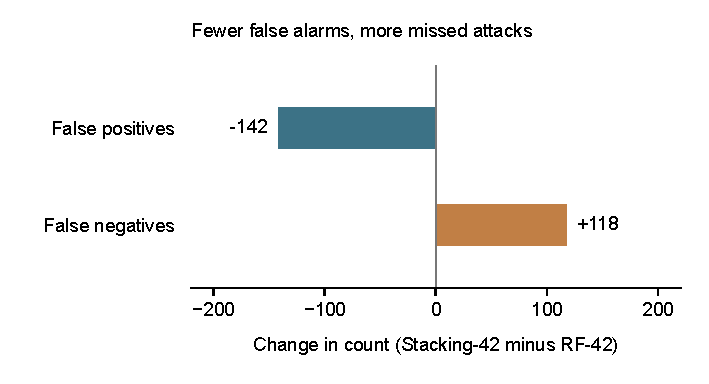
\includegraphics[width=0.82\textwidth]{../results/figures/p16_r05_error_tradeoff/error_tradeoff.pdf}
\caption{Chênh lệch số FP và FN của Stacking-42 so với RF-42 trên cùng official TEST.}
\label{fig:delta-fp-fn}
\end{figure}

\section{Độ bất định của chênh lệch và kiểm định cặp}
\label{sec:bat-dinh}

Bảng~\ref{tab:chenh-lech-ci} trình bày hiệu số Stacking-42 trừ RF-42 cùng khoảng tin cậy paired bootstrap 95\%. CI của Macro-F1 và MCC chứa 0; do đó, dữ liệu chưa cho thấy bằng chứng đủ rõ về ưu thế của Stacking trên hai chỉ số tổng hợp, nhưng cũng không thiết lập tương đương thống kê. McNemar exact sau hiệu chỉnh Holm cho ba cặp mô hình trong view đánh giá tương ứng cho $p_{\mathrm{Holm}}=0.468377$ đối với tính đúng tổng thể. Phép kiểm định này không kiểm định trực tiếp hiệu số Macro-F1.

\begin{table}[htbp]
\centering
\small
\renewcommand{\arraystretch}{1.3}
\setlength{\tabcolsep}{10pt}
\caption{Hiệu số Stacking-42 trừ RF-42 và CI 95\% paired bootstrap trên official TEST; hiệu số ở thang 0--1.}
\label{tab:chenh-lech-ci}
\begin{tabularx}{\linewidth}{X S[table-format=+1.6] S[table-format=+1.6] S[table-format=+1.6]}
\toprule
Chỉ số & {$\Delta$} & {Cận dưới} & {Cận trên}\\
\midrule
Macro-F1 & +0.000497 & -0.000312 & +0.001309\\
MCC & -0.000413 & -0.001938 & +0.001140\\
FPR & -0.003838 & -0.005243 & -0.002432\\
FNR & +0.002603 & +0.001853 & +0.003375\\
\bottomrule
\end{tabularx}
\end{table}

Các khoảng được tạo bằng 10\,000 lượt bootstrap phân tầng theo nhãn, seed 20260928, lấy mẫu theo các mẫu hình dự đoán liên hợp trên cùng dòng. CI percentile được tính riêng cho từng chỉ số; không có điều chỉnh đồng thời cho toàn bộ họ chỉ số. Hai CI lỗi cho thấy FPR thấp hơn và FNR cao hơn ở Stacking trong phép lấy mẫu lại này. Đây là bất định theo các dòng benchmark đã có dự đoán, không phản ánh biến thiên do huấn luyện lại, phụ thuộc session/host hay dữ liệu ngoài UNSW-NB15.

\begin{figure}[htbp]
\centering
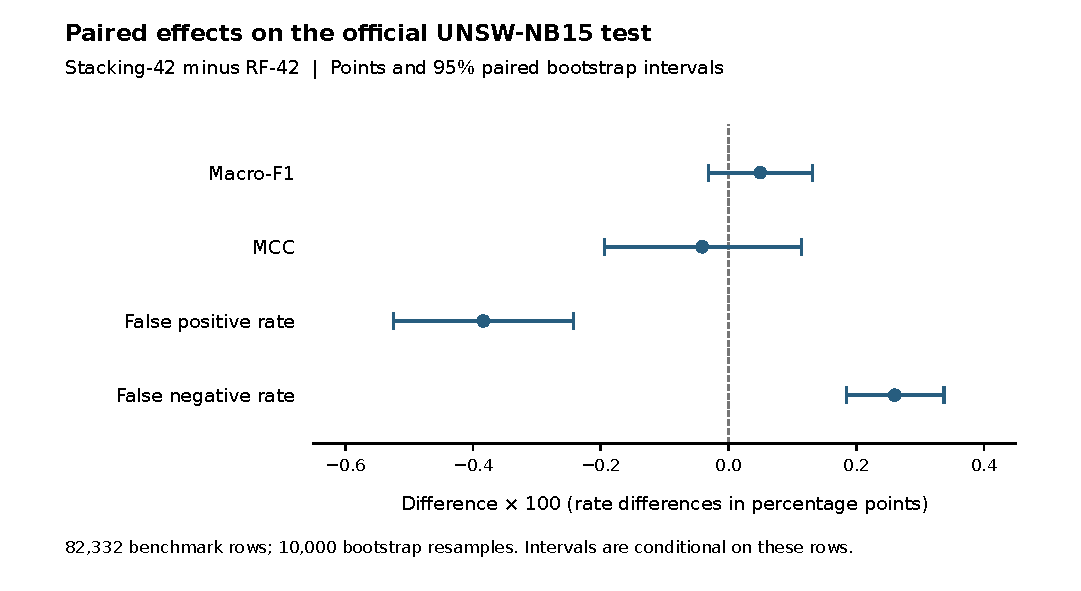
\includegraphics[width=0.95\textwidth]{../results/figures/p16_paired_effects_2026_10_16/paired_effects.pdf}
\caption{Hiệu số Stacking-42 trừ RF-42 và CI 95\% paired bootstrap; trục hoành thể hiện hiệu số nhân 100.}
\label{fig:paired-metrics}
\end{figure}

\section{Chi phí quan sát trong lần chạy lịch sử}
\label{sec:chi-phi}

Bảng~\ref{tab:chi-phi} đối chiếu thời gian huấn luyện, thời gian suy luận trung bình theo lô và dung lượng mô hình ước tính trong lần thực nghiệm ban đầu. Các con số cho thấy Stacking cần nhiều thời gian huấn luyện hơn RF-42 trong lần chạy đó, còn RF-17 có thời gian và kích thước thấp hơn. Chúng mô tả các cấu hình và môi trường lịch sử cụ thể; không phải benchmark lặp lại trên thiết bị triển khai.

\begin{table}[htbp]
\centering
\small
\renewcommand{\arraystretch}{1.3}
\setlength{\tabcolsep}{6pt}
\caption{Chi phí tính toán của ba pipeline trong lần thực nghiệm ban đầu; dung lượng quy đổi sang MiB.}
\label{tab:chi-phi}
\begin{tabularx}{\linewidth}{>{\raggedright\arraybackslash}X S[table-format=2.0] S[table-format=4.3] S[table-format=1.6] S[table-format=3.3]}
\toprule
Pipeline & {\shortstack{Số biến\\gốc}} & {\shortstack{Huấn luyện\\(s)}} & {\shortstack{Suy luận theo lô\\(ms/flow)}} & {\shortstack{Dung lượng\\(MiB)}}\\
\midrule
RF-42 & 42 & 371.244 & 0.008679 & 205.490\\
Stacking-42 & 42 & 980.170 & 0.012445 & 206.216\\
RF-17 & 17 & 57.255 & 0.003562 & 105.044\\
\bottomrule
\end{tabularx}
\par\vspace{4pt}
\begin{minipage}{\linewidth}\footnotesize
\emph{Ghi chú về chi phí lịch sử:} Các số giây phản ánh thời gian \textbf{fit riêng từng mô hình trong pipeline lịch sử} với cấu hình RF17 và RF42 khác nhau; \textbf{chưa bao gồm chi phí chọn stable17 từ đầu}. Log tài nguyên chuẩn về model CPU, RAM, mức song song thực tế và phiên bản môi trường gốc chưa đầy đủ; không suy ra chắc chắn cấu hình đa luồng. Các số này không phải đối chứng matched hoặc thời gian huấn luyện end-to-end, và không đối chiếu tốc độ tuyệt đối với P21.
\end{minipage}
\end{table}

Trong cùng đợt thực nghiệm, thời gian huấn luyện RF-42 gấp khoảng 6.48 lần RF-17; kích thước ước lượng của RF-17 thấp hơn khoảng 48.88\%. Trường suy luận là thời gian trung bình trên một dòng khi xử lý batch đã đánh giá, không phải độ trễ của một yêu cầu riêng lẻ. Môi trường thư viện gốc chưa được xác định trực tiếp, và kích thước được báo cáo không chứng minh artifact mô hình lịch sử hiện còn tồn tại.

\section{Sai số theo họ tấn công}
\label{sec:attack-family-error}

Phân tích hậu nghiệm theo họ nhãn thật làm rõ khác biệt mà chỉ số tổng thể gộp lại. Trong số 6\,062 mẫu Fuzzers, Stacking-42 bỏ sót 754 mẫu, nhiều hơn RF-42 (621); với Generic, số bỏ sót của Stacking thấp hơn (14 so với 57). Bảng~\ref{tab:attack-family} mở rộng đối chiếu tới đủ chín nhóm Attack và cả ba pipeline. FNR và số FN được nêu trong Bảng~\ref{tab:attack-family}, còn khoảng tin cậy Wilson 95\% được tách riêng tại Bảng~\ref{tab:attack-family-wilson} để bảo đảm kích thước chữ khi in khổ A4.

\begin{table}[htbp]\centering
\small\renewcommand{\arraystretch}{1.30}
\setlength{\tabcolsep}{5pt}
\caption{Số tấn công bỏ sót (FN) và FNR theo chín họ Attack trên official TEST; mỗi ô: \textbf{FN / FNR (\%)}.}
\label{tab:attack-family}
\begin{tabularx}{\linewidth}{@{}>{\raggedright\arraybackslash}p{3.2cm}r*{3}{>{\centering\arraybackslash}X}@{}}
\toprule
Họ Attack & $n$ & Stacking-42 & RF-42 & RF-17\\
\midrule
Analysis & 677 & 19 / 2.81\% & 3 / 0.44\% & 1 / 0.15\%\\
Backdoor & 583 & 1 / 0.17\% & 0 / 0.00\% & 0 / 0.00\%\\
DoS & 4089 & 9 / 0.22\% & 4 / 0.10\% & 2 / 0.05\%\\
Exploits & 11132 & 49 / 0.44\% & 45 / 0.40\% & 54 / 0.49\%\\
Fuzzers & 6062 & 754 / 12.44\% & 621 / 10.24\% & 623 / 10.28\%\\
Generic & 18871 & 14 / 0.07\% & 57 / 0.30\% & 3 / 0.02\%\\
Reconnaissance & 3496 & 2 / 0.06\% & 1 / 0.03\% & 19 / 0.54\%\\
Shellcode & 378 & 3 / 0.79\% & 2 / 0.53\% & 6 / 1.59\%\\
Worms & 44 & 1 / 2.27\% & 1 / 2.27\% & 0 / 0.00\%\\
\bottomrule
\end{tabularx}
\end{table}

\begin{table}[htbp]\centering
\small\renewcommand{\arraystretch}{1.23}
\setlength{\tabcolsep}{5pt}
\caption{Khoảng tin cậy Wilson 95\% cho FNR (\%) của cùng chín họ Attack. Đây là CI biên theo nhóm, không phải kiểm định paired giữa mô hình.}
\label{tab:attack-family-wilson}
\begin{tabularx}{\linewidth}{@{}>{\raggedright\arraybackslash}p{3.2cm}r*{3}{>{\centering\arraybackslash}X}@{}}
\toprule
Họ Attack & $n$ & Stacking-42 & RF-42 & RF-17\\
\midrule
Analysis & 677 & [1.80; 4.34] & [0.15; 1.29] & [0.03; 0.83]\\
Backdoor & 583 & [0.03; 0.97] & [0.00; 0.65] & [0.00; 0.65]\\
DoS & 4089 & [0.12; 0.42] & [0.04; 0.25] & [0.01; 0.18]\\
Exploits & 11132 & [0.33; 0.58] & [0.30; 0.54] & [0.37; 0.63]\\
Fuzzers & 6062 & [11.63; 13.29] & [9.51; 11.03] & [9.54; 11.07]\\
Generic & 18871 & [0.04; 0.12] & [0.23; 0.39] & [0.01; 0.05]\\
Reconnaissance & 3496 & [0.02; 0.21] & [0.01; 0.16] & [0.35; 0.85]\\
Shellcode & 378 & [0.27; 2.31] & [0.15; 1.91] & [0.73; 3.42]\\
Worms & 44 & [0.40; 11.81] & [0.40; 11.81] & [0.00; 8.03]\\
\bottomrule
\end{tabularx}
\end{table}

Hai bảng mô tả FN và khoảng tin cậy của FNR trong từng nhóm nhãn thật trên cùng official TEST, không phải độ chính xác của bộ phân loại đa lớp. Khoảng Wilson là khoảng nhị thức biên theo từng nhóm và pipeline; không phải kiểm định cặp giữa hai mô hình. Những nhóm hiếm, đặc biệt Worms, có khoảng rộng nên tỷ lệ quan sát được cần được đọc thận trọng. Các khác biệt theo nhóm gợi ý vị trí cần khảo sát thêm, nhưng không xác định đặc trưng hay cơ chế nào gây ra lỗi.

\section{Độ nhạy trên exact-duplicate-filtered subset}
\label{sec:exact-duplicate-filtered}

Trong official TEST có 8\,541 dòng mang \emph{vector 42 đặc trưng gốc giống hệt} ít nhất một vector TRAIN; sau khi lọc các dòng này còn 73\,791 dòng để tạo \emph{exact-duplicate-filtered view}. Ở đây, 'duplicate' chỉ có nghĩa là khớp toàn bộ 42 biến predictor, \textbf{không đồng nghĩa} cùng bản ghi gốc, session, thời điểm hoặc một cuộc tấn công mới. Bảng~\ref{tab:rev-rq4} so sánh Macro-F1 giữa official TEST và subset này, đồng thời báo cáo trực tiếp độ giảm. Đây là một view con của cùng holdout, không phải tập kiểm thử độc lập. Các giá trị giảm ở cả ba pipeline và thứ hạng theo Macro-F1 không đổi, nhưng phép lọc exact-vector không kiểm tra độc lập theo thời gian, host hoặc session. Vì vậy, nó cung cấp một phân tích độ nhạy hữu ích trong benchmark hiện có chứ chưa trả lời đầy đủ khả năng khái quát ngoài split chính thức.

\section{Bằng chứng phát triển mô hình: OOF, Voting và diversity}
\label{sec:revision-development}

Trước khi khóa ba pipeline cuối, các phương án kết hợp được khảo sát bằng dự đoán pooled out-of-fold trên official TRAIN. Bảng~\ref{tab:rev-dev} tập hợp kết quả của Random Forest và hai dạng Voting cùng Stacking trên track 42 đặc trưng. Outer cross-validation dùng \texttt{StratifiedKFold} ba fold với seed 42; tầng Stacking tạo dự đoán ngoài fold bằng inner cross-validation ba fold với seed 137.

\begin{table}[htbp]
\centering
\small
\renewcommand{\arraystretch}{1.28}
\setlength{\tabcolsep}{7pt}
\caption{Kết quả pooled OOF trong giai đoạn phát triển trên track 42 đặc trưng. FPR và FNR tính theo phần trăm.}
\label{tab:rev-dev}
\begin{tabularx}{\linewidth}{X S[table-format=1.6] S[table-format=1.6] S[table-format=2.4] S[table-format=1.4]}
\toprule
Cấu hình & {Macro-F1} & {MCC} & {FPR (\%)} & {FNR (\%)}\\
\midrule
Random Forest & 0.950387 & 0.901580 & 9.4214 & 1.8217\\
Hard Voting (LR/DT/RF) & 0.947325 & 0.896278 & 10.9357 & 1.4530\\
Soft Voting (LR/DT/RF) & 0.946758 & 0.894101 & 9.5232 & 2.2457\\
Stacking (LR/DT/RF) & 0.951484 & 0.903201 & 8.0536 & 2.3688\\
\bottomrule
\end{tabularx}

\par\vspace{4pt}
\begin{minipage}{\linewidth}
\footnotesize\emph{Lưu ý về selection bias ở giai đoạn lịch sử:} Bảng này chỉ hiển thị development OOF \textbf{track 42 biến gốc}; không phải bảng OOF riêng của RF17. Tuy nhiên \textbf{track stable17 lịch sử} được chọn bằng nhãn toàn official TRAIN \emph{trước} development CV, nên các ước lượng CV dùng track stable17 đó không đạt fully-nested feature selection và có thể lạc quan. Thí nghiệm P21 đánh giá feature selection theo FIT-only matched được trình bày riêng tại Bảng~\ref{tab:p21-five-arm-results}; không được dùng để sửa lại số liệu OOF lịch sử.
\end{minipage}
\end{table}

Trong giai đoạn phát triển, Stacking đạt Macro-F1 cao hơn RF 0.001097 và MCC cao hơn 0.001621; đồng thời FPR thấp hơn 1.3678 điểm phần trăm nhưng FNR cao hơn 0.5471 điểm. Hard và Soft Voting đều thấp hơn RF về Macro-F1 và MCC. Những chênh lệch này mô tả hiệu quả trên các dự đoán OOF đã lưu, song không phải kết quả holdout cuối và không cho biết liệu cùng thứ hạng có lặp lại qua nhiều lần huấn luyện hay không. Hơn nữa, tập đặc trưng stable17 được xác định trên toàn bộ TRAIN trước outer CV, còn việc tinh chỉnh meta learner chưa hoàn toàn nested; vì vậy các điểm phát triển có thể lạc quan.

Các cặp base learner cũng mắc lỗi không hoàn toàn trùng nhau: LR/RF có double-fault 0.030814 và tương quan lỗi 0.563855; DT/RF lần lượt là 0.025345 và 0.498922. Mức bổ sung lỗi này tạo điều kiện để một bộ kết hợp có thể khai thác khác biệt giữa các learner, nhưng tự nó không bảo đảm Voting hoặc Stacking sẽ cải thiện dự đoán. Kết quả Voting thấp hơn RF trong bảng là một minh họa trực tiếp cho sự phân biệt giữa diversity quan sát được và lợi ích thực tế của phép kết hợp.

\section{Đối chiếu các câu hỏi nghiên cứu}
\label{sec:revision-rq-all}

\subsection{RQ1: Ensemble có cải thiện ổn định so với mô hình đơn?}
\label{sec:revision-rq1}
Ở pooled OOF của track 42 biến, Stacking-42 nhỉnh hơn RF-42 về Macro-F1; trên official TEST chênh lệch Macro-F1 chỉ là $+0.000497$, trong khi MCC thấp hơn $0.000413$. CI paired bootstrap 95\% tương ứng là $[-0.000312;\,0.001309]$ và $[-0.001938;\,0.001140]$, đều chứa 0. McNemar exact sau hiệu chỉnh Holm cho $p=0.468377$ khi so sánh tính đúng tổng thể. Các kết quả này chưa cho thấy ưu thế tổng thể rõ của Stacking trên benchmark, nhưng cũng không chứng minh hai pipeline tương đương. So với RF-42, Stacking-42 giảm 142 FP và tăng 118 FN trong 82\,332 dự đoán.

Khoảng tin cậy được tính bằng lấy mẫu lại các dòng dự đoán đã ghép cặp; chúng không mô tả độ biến thiên giữa các lần fit độc lập. Ba artifact được tái dựng trên toàn TRAIN cũng không thay thế một nghiên cứu repeated-training. Do đó, \emph{ở giai đoạn đánh giá TEST lịch sử}, tính ổn định qua seed và lần huấn luyện vẫn chưa được xác định; phần bổ sung P21 phía dưới cung cấp phép khảo sát mới trên TRAIN-derived validation.

\noindent\textbf{Bổ sung hậu nghiệm P21 cho RQ1.}
Trong năm lần fit dùng 60\,000 hàng mỗi seed và chung 35\,069 hàng internal validation, RF42-Lite đạt Macro-F1 $0.945220$ (SD $0.000399$), còn Stacking-Lite đạt $0.944731$ (SD $0.000340$). Hiệu số Stacking trừ RF theo cặp trung bình $-0.000488$ (SD $0.000437$), FNR tăng trung bình $0.173$ điểm phần trăm, FPR giảm $0.213$ điểm. Chỉ có một trong năm seed cho hiệu số Macro-F1 dương rất nhỏ. Các cấu hình P21 khác cấu hình official TEST cũ; năm seed cùng một internal validation không tạo năm TEST độc lập. Bảng~\ref{tab:p21-five-arm-results} báo cáo đầy đủ các arm.

\subsection{RQ2: Feature Selection thay đổi chất lượng và chi phí ra sao?}
\label{sec:revision-rq2}
RF-17 đạt Macro-F1 0.860673 và MCC 0.746881, thấp hơn RF-42 (0.863343 và 0.750910). Số FN giảm từ 734 xuống 708, trong khi FP tăng từ 10\,003 lên 10\,224. Các số đo \emph{chỉ cho thời gian model fit lịch sử} cho thấy RF-17 cần 57.255 giây và có kích thước ước lượng 105.044 MiB; RF-42 lần lượt là 371.244 giây và 205.490 MiB. Những phép đo này chưa bao gồm chi phí tìm ra stable17 và không chứng minh lợi ích end-to-end của Feature Selection. Như vậy, hai cấu hình thể hiện đánh đổi giữa chất lượng, hai loại lỗi, thời gian và dung lượng.

Không thể quy các chênh lệch này riêng cho Feature Selection: RF-17 đồng thời dùng 150 cây và \texttt{min\_samples\_leaf}=2, còn RF-42 dùng 300 cây và giá trị 1. Hơn nữa, việc chọn stable17 trên toàn TRAIN trước development CV có thể làm điểm CV lạc quan. \emph{Đối với hai pipeline lịch sử}, RQ2 chưa cô lập được tác động riêng của số đặc trưng; phép đối chứng matched trên TRAIN-derived validation được bổ sung ở P21.

\noindent\textbf{Bổ sung hậu nghiệm P21 cho RQ2.}
Trong đối chứng matched, RF17-Lite và RF42-Lite đều có 150 cây, leaf=2, max-features=0.5, cùng FIT rows và seed. Bộ chọn 17 feature MI/L1/ExtraTrees được fit mới trên từng tập FIT (15 lượt selector trên 35\,000 hàng/seed; 14/17 feature xuất hiện ở cả năm lần). Macro-F1 trung bình RF17 là $0.936751$, kém RF42 $0.945220$; hiệu số paired $-0.008468$ (SD $0.001594$), MCC thấp hơn $0.016939$, FNR cao hơn $0.534$ điểm phần trăm. Nếu \emph{sử dụng tập feature đã cố định} từ lượt chọn trước thì riêng khâu fit RF17 trung bình $84.600$ giây so với $241.119$ giây ở RF42 ($2.85$ lần nhanh hơn); cộng thời gian chọn biến trung bình $225.250$ giây, tổng \emph{selection + RF17 fit} là $309.850$ giây, \emph{cao hơn} chi phí fit RF42 $241.119$ giây. Đây không phải một so sánh độ trễ suy luận hay hiệu năng trên official TEST.

\subsection{RQ3: Diversity lỗi có liên hệ thế nào với kết quả Ensemble?}
\label{sec:revision-rq3}
Các cặp learner trong development có lỗi bổ sung, nhưng hai phương án Voting không vượt RF về Macro-F1. Stacking chỉ cao hơn RF một mức nhỏ ở pooled OOF, và ưu thế đó không rõ trên official TEST. Phân tích paired correctness cuối cùng cho thấy 71\,104 mẫu cả RF-42 và Stacking-42 đều dự đoán đúng, 10\,222 mẫu cả hai cùng sai, 491 mẫu RF đúng/Stacking sai và 515 mẫu RF sai/Stacking đúng. Hai loại bất đồng gần cân bằng, phù hợp với kết quả McNemar không cho thấy khác biệt rõ về tính đúng tổng thể.

Paired correctness của hai mô hình cuối không đồng nhất với diversity giữa các base learner trong development. Cả hai phân tích đều mang tính mô tả; chúng cho thấy có khác biệt về lỗi để khảo sát, nhưng chưa xác định cơ chế nhân quả khiến phép kết hợp sửa hay tạo thêm một lỗi cụ thể.

\subsection{RQ4: Hiệu năng thay đổi ra sao khi loại các vector TEST trùng TRAIN?}
\label{sec:revision-rq4}
Trong 82\,332 dòng official TEST, có 8\,541 dòng trùng một vector 42 đặc trưng với ít nhất một vector TRAIN. Khi loại các dòng này, Macro-F1 giảm ở cả ba pipeline; Bảng~\ref{tab:rev-rq4} cho thấy mức giảm nhỏ và thứ hạng giữa các cấu hình không đổi theo chỉ số này.

\begin{table}[htbp]
\centering
\small
\renewcommand{\arraystretch}{1.3}
\setlength{\tabcolsep}{9pt}
\caption{Macro-F1 trên official TEST và exact-duplicate-filtered subset thuộc cùng tập kiểm thử.}
\label{tab:rev-rq4}
\begin{tabularx}{\linewidth}{X S[table-format=1.6] S[table-format=1.6] S[table-format=+1.6]}
\toprule
Pipeline & {Official TEST} & {Exact-duplicate-filtered} & {$\Delta$}\\
\midrule
Stacking-42 & 0.863840 & 0.858125 & -0.005715\\
RF-42 & 0.863343 & 0.857473 & -0.005870\\
RF-17 & 0.860673 & 0.855723 & -0.004950\\
\bottomrule
\end{tabularx}
\end{table}

Khoảng cách Macro-F1 giữa Stacking-42 và RF-42 vẫn nhỏ trong cả hai view. Exact-duplicate-filtered là phân tích độ nhạy trên chính official TEST, được xác định theo trùng khớp chính xác của vector đặc trưng; nó không thay thế đánh giá theo thời gian, host, session hay benchmark ngoài. Vì vậy RQ4 chỉ được trả lời trong phạm vi phép lọc vector này, chưa xác lập khả năng khái quát sang dữ liệu độc lập.

\subsection{RQ5: Xử lý mất cân bằng ảnh hưởng thế nào đến lỗi?}
\label{sec:revision-rq5}
Official TRAIN gồm 56\,000 Normal (31.94\%) và 119\,341 Attack (68.06\%); official TEST gồm 37\,000 Normal (44.94\%) và 45\,332 Attack (55.06\%). Trên TEST, RF-42 có FPR 27.0351\% và FNR 1.6192\%; Stacking-42 lần lượt là 26.6514\% và 1.8795\%; RF-17 là 27.6324\% và 1.5618\%. Những chỉ số này mô tả đánh đổi lỗi theo lớp, đồng thời phân tích theo họ tấn công cho thấy mức bỏ sót không đồng đều giữa các nhóm có quy mô rất khác nhau.

Trong quá trình tinh chỉnh đã có so sánh \texttt{class\_weight=None} với \texttt{balanced} cho meta learner, và cấu hình Stacking cuối dùng \texttt{None}. Tuy nhiên, không có đối chứng matched giữa weighting và không weighting, hoặc giữa resampling và không resampling trong cùng một protocol. Kết quả official TEST lịch sử này không cô lập được ảnh hưởng riêng của weighting/resampling; P21 sau đó bổ sung đối chứng matched chỉ trong official TRAIN, trình bày riêng phía dưới.

\noindent\textbf{Bổ sung hậu nghiệm P21 cho RQ5.}
Normal mới là lớp ít mẫu trong TRAIN (56\,000 so với 119\,341 Attack). Trong năm lần FIT-matched trên TRAIN-derived internal validation, \texttt{class\_weight=balanced} ở RF42 giảm FPR $3.164$ điểm phần trăm nhưng tăng FNR $1.788$ điểm so với RF42 không cân bằng; Macro-F1 giảm $0.001343$. Oversampling ngẫu nhiên \emph{chỉ trên FIT Normal} giảm FPR $2.209$ điểm và tăng FNR $1.168$ điểm; Macro-F1 giảm trung bình $0.000334$. Cả hai nhánh giảm cảnh báo giả nhưng làm bỏ sót nhiều Attack hơn trong đánh giá này, không có điều chỉnh ngưỡng hậu nghiệm.

\noindent\textbf{Tổng hợp cập nhật RQ1--RQ5.} Phần official TEST lịch sử và thí nghiệm bổ sung P21 là hai phạm vi dữ liệu, giả thuyết và cấu hình khác nhau, không được gộp để suy ra kiểm định thống kê. Trên P21, RQ1 không ghi nhận lợi thế Macro-F1 nhất quán cho Stacking-Lite; RQ2 ghi nhận FIT riêng RF17 nhanh hơn nhưng Macro-F1 giảm và tổng thời gian tính cả selection tăng; RQ5 cho thấy weighting và oversampling giảm FPR nhưng tăng FNR. RQ3 vẫn chỉ cho bằng chứng diversity mang tính mô tả; RQ4 vẫn chỉ là phép lọc exact-duplicate-filtered của official TEST lịch sử, không phải benchmark mới. Các bằng chứng P21 là \emph{post-hoc reused-TRAIN internal validation}, không phải kết quả TEST độc lập.

\section{P21: Kết quả đối chứng hậu nghiệm trên internal validation của TRAIN}
\label{sec:p21-results}
Báo cáo kết quả bổ sung này được tạo \emph{sau} quá trình đánh giá official TEST lịch sử. Năm seed tạo năm tập FIT 60\,000 dòng khác nhau nhưng tất cả dự đoán trên \textbf{cùng} 35\,069 dòng internal validation của official TRAIN (11\,200 Normal và 23\,869 Attack). Đây không phải năm lần đánh giá độc lập trên TEST hoặc một benchmark ngoài. Tất cả 25 lượt fit (5 arm $\times$ 5 seed) đều hoàn tất, với checksum nguồn dữ liệu và cấu hình khớp, confusion matrix được kiểm tra lại, không truy cập official TEST khi chạy P21.

\begin{table}[htbp]\centering
\small
\renewcommand{\arraystretch}{1.26}
\setlength{\tabcolsep}{3pt}
\caption{Hiệu năng trung bình qua 5 FIT seed trên \textbf{một} internal validation P21; độ lệch chuẩn mẫu \emph{có điều kiện trên cùng validation} của Macro-F1 và MCC ghi trong ngoặc. FPR/FNR tính bằng phần trăm.}
\label{tab:p21-five-arm-results}
\begin{tabular}{lrrrr}
\toprule
Arm P21 & \shortstack{Macro-F1\\(SD theo FIT)} & \shortstack{MCC\\(SD theo FIT)} & FPR (\%) & FNR (\%)\\\midrule
RF42-Lite (A0) & \shortstack{0.945220\\{\scriptsize (0.000399)}} & \shortstack{0.890971\\{\scriptsize (0.000858)}} & 9.6196 & 2.3989\\
RF17-Lite (A1) & \shortstack{0.936751\\{\scriptsize (0.001291)}} & \shortstack{0.874032\\{\scriptsize (0.002462)}} & 10.7589 & 2.9327\\
RF42 Balanced (A2) & \shortstack{0.943877\\{\scriptsize (0.000275)}} & \shortstack{0.887909\\{\scriptsize (0.000563)}} & 6.4554 & 4.1870\\
RF42 Oversample (A3) & \shortstack{0.944886\\{\scriptsize (0.000742)}} & \shortstack{0.889776\\{\scriptsize (0.001480)}} & 7.4107 & 3.5670\\
Stacking-Lite (A4) & \shortstack{0.944731\\{\scriptsize (0.000340)}} & \shortstack{0.889864\\{\scriptsize (0.000738)}} & 9.4071 & 2.5715\\\bottomrule
\end{tabular}
\vspace{3pt}

\begin{minipage}{\linewidth}
\footnotesize\emph{Lưu ý phương pháp luận:} SD ở đây chỉ phản ánh biến thiên khi thay đổi tập FIT và seed trong khi giữ \textbf{cùng một tập validation 35\,069 dòng}. Đây không phải SD của năm benchmark độc lập, cũng không ước lượng sai số tổng quát hóa trên traffic mới. Không sử dụng năm giá trị này như năm tập TEST độc lập để làm t-test/ANOVA hoặc tuyên bố độ ổn định ngoài phân bố.
\end{minipage}
\end{table}

\begin{table}[htbp]\centering
\small
\renewcommand{\arraystretch}{1.24}
\setlength{\tabcolsep}{3pt}
\caption{Hiệu số \emph{paired FIT seed} của mỗi arm so với RF42-Lite A0; dấu của $\Delta$ là arm $-$ A0. $\Delta$ FPR/FNR tính bằng \emph{điểm phần trăm}, không phải \%.}
\label{tab:p21-paired-deltas}
\begin{tabular}{lrrrr}
\toprule
So sánh & $\Delta$ Macro-F1 & $\Delta$ MCC & $\Delta$ FPR (đpp) & $\Delta$ FNR (đpp)\\\midrule
A1 $-$ A0 & $-0.008468$ & $-0.016939$ & $+1.1393$ & $+0.5337$\\
A2 $-$ A0 & $-0.001343$ & $-0.003062$ & $-3.1643$ & $+1.7881$\\
A3 $-$ A0 & $-0.000334$ & $-0.001195$ & $-2.2089$ & $+1.1680$\\
A4 $-$ A0 & $-0.000488$ & $-0.001107$ & $-0.2125$ & $+0.1726$\\\bottomrule
\end{tabular}
\end{table}

\subsection{Độ biến thiên giữa năm FIT seed}
Năm Macro-F1 của RF42-Lite lần lượt là 0.944741; 0.945712; 0.945546; 0.945080; 0.945019. Tương ứng, Stacking-Lite lần lượt là 0.944444; 0.944559; 0.945079; 0.945121; 0.944454. Hiệu số paired của Stacking trừ RF là $[-0.000297;\,-0.001153;\,-0.000468;\,+0.000041;\,-0.000565]$; có một seed nhỉnh hơn rất nhỏ nhưng không làm đảo dấu hiệu số trung bình.

\begin{table}[htbp]\centering
\small
\renewcommand{\arraystretch}{1.25}
\setlength{\tabcolsep}{7pt}
\caption{Macro-F1 theo FIT seed, chỉ mô tả biến thiên huấn luyện có điều kiện; \textbf{cùng} 35\,069 quan sát validation ở cả năm cột.}
\label{tab:p21-by-seed}
\begin{tabular}{lrrrrr}
\toprule
Arm & 1103 & 2207 & 3301 & 4409 & 5501\\\midrule
A0 RF42 & 0.944741 & 0.945712 & 0.945546 & 0.945080 & 0.945019\\
A1 RF17 & 0.938678 & 0.935777 & 0.936491 & 0.935483 & 0.937328\\
A2 Balanced & 0.944006 & 0.943785 & 0.944231 & 0.943877 & 0.943485\\
A3 Oversample & 0.944235 & 0.945297 & 0.944752 & 0.944201 & 0.945945\\
A4 Stacking & 0.944444 & 0.944559 & 0.945079 & 0.945121 & 0.944454\\\bottomrule
\end{tabular}
\end{table}

\subsection{RQ1: Ensemble và đánh đổi lỗi}
Stacking-Lite (A4) không tăng Macro-F1/MCC trung bình so với RF42-Lite (A0) trên năm seed; chênh lệch trung bình lần lượt $-0.000488$ và $-0.001107$. Đồng thời FPR giảm 0.2125 điểm phần trăm, FNR tăng 0.1726 điểm. Đây là khác biệt nhỏ trong \emph{cấu hình Lite} được khống chế; nó không bác bỏ lợi ích của mọi cấu trúc ensemble. Không kết luận tương đương thống kê dựa trên năm seed có chung tập validation.

\subsection{RQ2: Đối chứng matched Feature Selection và chi phí thực tế}
A1 và A0 sử dụng cùng siêu tham số RF, số FIT rows và seed; biến duy nhất trong \emph{mô hình RF} là track 17 thay cho 42 đặc trưng gốc, song toàn bộ pipeline A1 cần bước chọn biến mới. Có 14 đặc trưng xuất hiện trong cả năm bộ top-17, gồm \texttt{ct\_srv\_dst}, \texttt{ct\_state\_ttl}, \texttt{dload}, \texttt{dttl}, \texttt{proto}, \texttt{state}, \texttt{sttl}, \texttt{ct\_dst\_ltm}, \texttt{dmean}, \texttt{dwin}, \texttt{rate}, \texttt{service}, \texttt{swin}, \texttt{is\_sm\_ips\_ports}.

\begin{table}[htbp]\centering\small
\renewcommand{\arraystretch}{1.22}
\caption{Chi phí huấn luyện trung bình theo năm FIT seed, đơn vị giây. Các số là thời gian fit ghi từ worker, không phải end-to-end latency triển khai.}
\label{tab:p21-cost}
\begin{tabular}{lr}\toprule
Công đoạn & Thời gian trung bình (s)\\\midrule
Chỉ fit RF42-Lite & 241.119\\
Chỉ fit RF17-Lite (sau chọn đặc trưng) & 84.600\\
Chọn stable17 từ FIT & 225.250\\
\textbf{Chọn stable17 + fit RF17-Lite} & \textbf{309.850}\\
Chỉ fit RF42 Balanced & 230.247\\
Chỉ fit RF42 Oversample & 355.197\\
Chỉ fit Stacking-Lite & 652.913\\\bottomrule
\end{tabular}
\end{table}
Nếu bỏ qua chi phí chọn feature, A1 fit RF nhanh hơn A0 khoảng 2.85 lần. Trong kịch bản \emph{phải tìm lại 17 đặc trưng cho mỗi lượt huấn luyện}, chi phí \emph{selection + RF fit} của A1 cao hơn khoảng 28.5\% so với riêng fit RF42 trong thiết kế P21. Cả hai tổng này chưa cộng thời gian xử lý dữ liệu ngoài các lời gọi đã đo, lưu artifact, giám sát hay latency phục vụ nên không được gọi là tổng chi phí triển khai end-to-end. Vì vậy không thể dựa vào thời gian fit RF17 để tuyên bố Feature Selection đã làm giảm \emph{tổng} chi phí training.

\subsection{RQ5: Cân bằng lớp không đồng nghĩa tăng phát hiện Attack}
Trên dữ liệu TRAIN, Normal là lớp ít mẫu và được tăng trọng số hoặc lặp lại trong hai nhánh can thiệp. A2 giảm FPR mạnh hơn A3 nhưng cũng làm FNR tăng mạnh hơn. So với A0, A2 giảm FPR 3.1643 điểm phần trăm, tăng FNR 1.7881 điểm; A3 giảm FPR 2.2089 điểm, tăng FNR 1.1680 điểm. Cả hai làm giảm Macro-F1 trung bình, cho thấy đánh đổi giữa cảnh báo giả và bỏ sót tấn công trong mô hình và benchmark nội bộ cụ thể này. Không chọn ngưỡng mới dựa vào validation đã đánh giá.

\subsection{Chất lượng bằng chứng và giới hạn phát biểu}
Mỗi seed có năm cấu hình trùng digest FIT source và cùng nhãn true 35\,069 dòng validation, các kiểm tra kết quả phát hiện tổng TN+FP+FN+TP đúng support, khớp các chỉ số Macro-F1/MCC/FPR/FNR và không cho thấy lệch dữ liệu trong metadata. Tuy nhiên đây là \emph{kiểm tra nhất quán báo cáo}, không phải replay độc lập trên máy thứ hai hay đối chứng theo thời gian. Cụm seed chỉ thay đổi mẫu FIT và tính ngẫu nhiên của mô hình; do validation được tái sử dụng, độ lệch chuẩn trong các bảng đo biến thiên \emph{có điều kiện trên validation đó}, không phải sai số tổng quát hóa. Số liệu P21 không được gộp với official TEST 82\,332 dòng của giai đoạn lịch sử để tính p-value hay chọn mô hình cuối.


\chapter{THẢO LUẬN VÀ HƯỚNG PHÁT TRIỂN}
\label{chap:ban-luan}
\section{Diễn giải đánh đổi giữa các loại lỗi}
\label{sec:discussion-error-tradeoff}

Trên cùng official TEST, Stacking-42 giảm 142 cảnh báo giả so với RF-42 nhưng bỏ sót thêm 118 mẫu Attack. Giá trị thực tế của thay đổi này phụ thuộc vào chi phí tương đối của cảnh báo giả và bỏ sót trong môi trường vận hành; chưa có dữ liệu thật về chi phí đó; phần phân tích độ nhạy giả định phía dưới chỉ minh họa điều kiện để hai pipeline đổi thứ hạng theo chi phí, không xếp một cấu hình là tối ưu cho mọi NIDS. Macro-F1 gần như không đổi và MCC giảm nhẹ ở Stacking, trong khi FPR và FNR dịch chuyển theo hai hướng khác nhau. Việc đọc đồng thời các chỉ số này cho thấy lý do một điểm tổng hợp duy nhất chưa đủ để quyết định triển khai.

Ma trận tính đúng/sai theo cặp dưới đây cho thấy số dự đoán bất đồng giữa hai pipeline gần cân bằng. Điều này phù hợp với McNemar không phát hiện khác biệt rõ về tính đúng tổng thể, nhưng không thay thế các chỉ số tách theo lớp hay thiết lập tương đương thống kê.

\begin{table}[htbp]
\centering
\small
\renewcommand{\arraystretch}{1.3}
\setlength{\tabcolsep}{14pt}
\caption{Tính đúng/sai theo cặp dự đoán của RF-42 và Stacking-42 trên official TEST.}
\label{tab:paired-correctness}
\begin{tabular}{l S[table-format=5.0] S[table-format=5.0]}
\toprule
 & {Stacking đúng} & {Stacking sai}\\
\midrule
RF đúng & 71104 & 491\\
RF sai & 515 & 10222\\
\bottomrule
\end{tabular}
\end{table}

\subsection{Phân tích độ nhạy chi phí báo động giả và bỏ sót tấn công}
\label{sec:v4-fp-fn-cost}
Để diễn giải đánh đổi trên official TEST \emph{lịch sử} mà không tự giả định chi phí thực tế của một trung tâm SOC, đặt chi phí mỗi cảnh báo giả $C_{\mathrm{FP}}>0$ và chi phí mỗi tấn công bị bỏ sót $C_{\mathrm{FN}}=r C_{\mathrm{FP}}$, với $r$ là \emph{tỷ lệ giả định}, không phải thông số được đo. Tổn thất chuẩn hóa tính theo số lỗi:
\[
L=\frac{C_{\mathrm{FP}}\cdot FP+C_{\mathrm{FN}}\cdot FN}{C_{\mathrm{FP}}}=FP+r FN.
\]
Từ confusion matrices trên \emph{cùng} 82\,332 dòng official TEST và ngưỡng phân loại khóa $0.5$, RF-42 có $FP=10\,003$, $FN=734$; Stacking-42 có $FP=9\,861$, $FN=852$. Do đó
\[
L_{\mathrm{RF}}=10\,003+734r,\quad
L_{\mathrm{Stack}}=9\,861+852r,\quad
L_{\mathrm{Stack}}-L_{\mathrm{RF}}=-142+118r.
\]
Hai mô hình có tổn thất bằng nhau khi $r=142/118\approx1.2034$. Nếu $r$ lớn hơn ngưỡng này, \textbf{RF-42 có tổn thất thấp hơn Stacking-42 \emph{trong đúng phép so sánh hai mô hình này}}; không suy ra RF-42 tối ưu hơn RF-17 hoặc mọi NIDS khác.

\begin{table}[htbp]\centering\small
\renewcommand{\arraystretch}{1.23}
\caption{Phân tích độ nhạy \emph{giả định} theo $r=C_{\mathrm{FN}}/C_{\mathrm{FP}}$, chuẩn hóa $C_{\mathrm{FP}}=1$. Giá trị là điểm tổn thất quy ước, không phải số tiền thiệt hại thực tế.}
\label{tab:v4-cost-sensitivity}
\begin{tabular}{rrrrl}\toprule
$r$ & $L_{\mathrm{RF}}$ & $L_{\mathrm{Stack}}$ & $L_{\mathrm{Stack}}-L_{\mathrm{RF}}$ & Tổn thất thấp hơn\\\midrule
1 & 10737 & 10713 & -24 & Stacking-42\\
5 & 13673 & 14121 & +448 & RF-42\\
10 & 17343 & 18381 & +1038 & RF-42\\
50 & 46703 & 52461 & +5758 & RF-42\\
100 & 83403 & 95061 & +11658 & RF-42\\\bottomrule
\end{tabular}
\end{table}

Bảng~\ref{tab:v4-cost-sensitivity} chỉ khảo sát một số tỷ lệ chi phí do người nghiên cứu \emph{định nghĩa để minh họa}, không có bằng chứng định lượng rằng $r=5$ hoặc $r=100$ đúng cho hệ thống tại Học viện. Mô hình cộng tuyến tính chưa xét mức độ nghiêm trọng từng tấn công, số cảnh báo lặp, khả năng xác minh của SOC, điều chỉnh ngưỡng hoặc chi phí drift; vì vậy đây là \textbf{phân tích độ nhạy của confusion matrix hiện có}, không phải kết quả tối ưu hóa chính sách vận hành hay dự đoán thiệt hại thực tế.


\section{Diversity và sai số theo nhóm}
\label{sec:discussion-diversity-families}

Các learner cơ sở mắc lỗi không hoàn toàn trùng nhau trong development, nhưng kết quả Hard/Soft Voting thấp hơn RF và lợi thế nhỏ của Stacking không rõ trên official TEST. Như vậy, diversity là một thuộc tính quan sát được của các dự đoán, còn lợi ích của ensemble phải được xác lập trực tiếp bằng hiệu năng và loại lỗi của bộ kết hợp. Paired correctness của hai pipeline cuối cũng chỉ mô tả bất đồng; nó không cho biết một base learner cụ thể đã gây ra hay sửa một lỗi nào.

Phân tích theo họ Attack cho thấy mức lỗi không đồng đều: chênh lệch giữa Stacking và RF-42 lớn hơn ở Fuzzers nhưng đi theo hướng ngược lại ở Generic (Bảng~\ref{tab:attack-family}). Vì các mô hình được huấn luyện cho Normal/Attack, đây là phân nhóm hậu nghiệm theo nhãn thật, không phải phép đánh giá đa lớp. Các biến như \texttt{sttl}, \texttt{proto} hay \texttt{state} có thể liên hệ với những dự đoán khác nhau, song dữ liệu mô tả không xác định được cơ chế nhân quả.

\section{Ý nghĩa và giới hạn của Feature Selection}
\label{sec:discussion-feature-selection}

RF-17 có thời gian huấn luyện và kích thước ước lượng thấp hơn RF-42, đi kèm Macro-F1 thấp hơn, ít FN hơn nhưng nhiều FP hơn. Đây là một đánh đổi có thể quan sát giữa hai pipeline. Vì số cây và kích thước lá cũng khác, chưa thể quy chênh lệch cho riêng việc giảm 25 biến. Bên cạnh đó, stable17 được chọn từ toàn bộ TRAIN trước development CV; điểm OOF do đó có thể lạc quan hơn đánh giá nested, dù official TEST không được dùng để tạo danh sách đặc trưng.

Phần official TEST lịch sử không thực hiện phép đối chứng matched này. P21 sau đó bổ sung hai RF với cùng 150 cây, leaf=2, max-features=0.5, cùng FIT source rows, selector FIT-only mới qua từng seed. Kết quả P21 được diễn giải riêng trong Mục~\ref{sec:p21-results}, không dùng để sửa lại kết quả official TEST lịch sử.

\section{Độ bất định và phạm vi suy luận}
\label{sec:discussion-uncertainty}

CI paired bootstrap 95\% của hiệu số Macro-F1 và MCC chứa 0, trong khi CI của FPR và FNR nằm ở hai phía đối nghịch. Cùng với McNemar trên tính đúng tổng thể, các kết quả ủng hộ cách diễn giải rằng Stacking làm thay đổi cơ cấu lỗi trên benchmark nhưng chưa thể hiện ưu thế tổng thể rõ. Không bác bỏ khác biệt không đồng nghĩa với chứng minh tương đương. Bootstrap lấy mẫu lại các dòng dự đoán đã ghép cặp và giữ tỷ lệ lớp; nó không tái tạo biến thiên từ quá trình huấn luyện, phụ thuộc giữa các flow, hay thay đổi giữa các mạng. Trong P21, SD giữa năm seed chỉ đo biến thiên FIT/seed có điều kiện trên một validation chung, không phải SD của năm mạng độc lập (Bảng~\ref{tab:p21-five-arm-results}).

Official TEST và exact-duplicate-filtered subset đều thuộc UNSW-NB15. Việc Macro-F1 giảm trên subset sau khi bỏ các vector trùng là bằng chứng về độ nhạy với định nghĩa view này; nó không đại diện temporal, host/session-separated hay external validation. Các khoảng Wilson trong Bảng~\ref{tab:attack-family-wilson} là ước lượng biên theo từng nhóm/pipeline, không phải kiểm định cặp; với các nhóm hiếm, khoảng rộng nhắc rằng tỷ lệ quan sát được còn kém chính xác.

\section{Tái lập, tái huấn luyện và triển khai}
\label{sec:discussion-reproducibility}

P15 đã tái dựng riêng RF-17, RF-42 và Stacking-42 trên toàn bộ 175\,341 dòng TRAIN trong môi trường Python 3.11.9 và scikit-learn 1.9.0. Việc kiểm tra hash, schema, khả năng nạp lại và tạo xác suất trên dòng TRAIN-derived hỗ trợ khả năng tái lập cấu hình trong môi trường phần mềm được xác định. Tuy vậy, do thiếu môi trường thư viện và đối tượng mô hình lịch sử, các artifact mới không được xem là đồng nhất với mô hình từng tạo ra điểm TEST.

Tái dựng trên TRAIN khác với xác minh lại kết quả TEST lịch sử; cả hai đều khác với đánh giá triển khai. Các metric của P9/P15 trong các phần lịch sử vẫn được giữ khóa; các con số P21 mới là thí nghiệm matched hậu nghiệm trên internal validation của TRAIN và được tách nhãn rõ. Việc mô hình có thể được fit, nạp và gọi dự đoán trong môi trường ghi nhận không cung cấp bằng chứng về độ trễ yêu cầu, tải xử lý, khả năng thích nghi với drift hay tính sẵn sàng vận hành của một NIDS.

\section{Tổng hợp câu trả lời nghiên cứu}
\label{sec:revision-rq-map}

Bảng~\ref{tab:rq-evidence} tóm tắt kết quả thực nghiệm có thể bảo vệ cùng phần còn chưa được xác định. Các khoảng trống được nêu trong mối liên hệ với kết quả, thay vì thay thế câu trả lời bằng danh sách giới hạn.

\begin{table}[htbp]
\centering
\small
\renewcommand{\arraystretch}{1.35}
\setlength{\tabcolsep}{6pt}
\caption{Kết luận thực nghiệm cho RQ1--RQ5 và phạm vi chưa được kiểm chứng.}
\label{tab:rq-evidence}
\begin{tabularx}{\linewidth}{p{0.9cm} X X}
\toprule
RQ & Kết luận trong phạm vi dữ liệu & Bằng chứng còn cần thiết\\
\midrule
RQ1 & Stacking-Lite không hơn RF42-Lite theo Macro-F1 trung bình qua năm FIT seed P21; TEST lịch sử cũng không chứng minh vượt trội. & Độ ổn định ngoài một validation dùng chung.\\
RQ2 & RF17 FIT nhanh hơn RF42 nhưng giảm Macro-F1 trong đối chứng matched P21; cộng chi phí chọn biến từ đầu còn chậm hơn. & Độ trễ dự đoán, bộ nhớ arm, chi phí khi triển khai.\\
RQ3 & Diversity lỗi xuất hiện ở learner cơ sở nhưng không bảo đảm Voting/Stacking có lợi. & Thiết kế kiểm tra cơ chế bổ sung lỗi thay vì tương quan mô tả.\\
RQ4 & Macro-F1 giảm trong exact-duplicate-filtered view; thứ hạng theo Macro-F1 được giữ. & Đánh giá theo thời gian/host/session hoặc benchmark ngoài.\\
RQ5 & Weighting/oversampling FIT-only được đối chiếu matched ở P21: cả hai giảm FPR và tăng FNR so với RF42. & Đánh giá threshold-cost và dữ liệu traffic độc lập.\\
\bottomrule
\end{tabularx}
\end{table}

\section{Hướng nghiên cứu tiếp theo}

P21 đã bổ sung năm lượt huấn luyện matched có kiểm soát seed, FIT-only feature selection và đối chứng class weighting/oversampling. Tuy nhiên các lượt fit vẫn chia sẻ \emph{một} internal validation, và được thiết kế sau khi biết kết quả TEST lịch sử. Hướng tiếp theo vì vậy là đánh giá theo thời gian, host/session hoặc benchmark mạng ngoài có quyền sử dụng rõ ràng, với kế hoạch tiền đăng ký trước khi xem kết quả; tiếp theo mới khảo sát threshold tối ưu theo chi phí báo động giả và bỏ sót thực tế. Những bước này không thay đổi kết quả official holdout cũ.


\section{Giới hạn bổ sung riêng cho thực nghiệm P21}
\label{sec:p21-validity}
P21 là một nhánh nghiên cứu hậu nghiệm. Lý do bổ sung đối chứng matched xuất phát từ các điểm yếu đã được nhận diện sau giai đoạn thử nghiệm chính; vì vậy không được gọi P21 là tiền đăng ký của toàn bộ công trình. Hai điều kiện phải được tách bạch: \emph{P21 không đọc official TEST khi fit/đánh giá} nhưng \emph{internal validation của TRAIN đã được chấm điểm}. Trường metadata \texttt{validation\_evaluation\_performed=false} nằm trong \emph{split audit trước khi fit}, không phủ định sự tồn tại của bảng metrics validation ở output cuối. Chỉ số P21 thuộc một partition cố định của TRAIN, không được xem là phép xác nhận ngoại sinh.

Các biến thể A0--A4 có cùng FIT source identities trong mỗi seed và cùng ngưỡng $0.5$. Điều đó hạn chế chênh lệch do mẫu nhưng không tự chứng minh các quan sát độc lập theo session/host; grouping dựa trên vector 42 biến chỉ chặn trường hợp trùng \emph{chính xác}, không phát hiện toàn bộ các flow liên quan. P21 sử dụng 5 FIT seed, nhưng tất cả cùng 35\,069 nhãn true nội bộ; không thể coi đó là $n=5$ tập benchmark độc lập hay tuyên bố khẳng định superiority bằng p-value. Phạm vi hợp lệ là đánh giá \emph{độ nhạy do tái chọn FIT và seed} trong một protocol cố định trên cùng internal validation.

Việc chỉ dùng 60\,000 dòng FIT cho từng seed P21 và RF42-Lite 150 cây khác với thí nghiệm trên toàn TRAIN và official TEST của ba model lịch sử; vì vậy độ chênh lệch FPR/FNR giữa hai giai đoạn chịu ảnh hưởng của phân bố dữ liệu, kích thước FIT, hyperparameters, tập đánh giá và thời điểm thiết kế. Không thể so sánh trực tiếp các giá trị tuyệt đối rồi gọi đó là cải thiện sau huấn luyện. RQ2 chỉ đo thời gian chọn biến và model fit; cần tính thêm lưu trữ model, tiền xử lý, predict latency và chi phí duy trì selector nếu muốn kết luận sẵn sàng triển khai.

\section{Kết luận}
\label{chap:ket-luan}
Nghiên cứu đánh giá học tổ hợp và mô hình đơn cho phân loại nhị phân Normal/Attack trên UNSW-NB15 bằng hai lớp bằng chứng được tách biệt về thời điểm thiết kế và bộ dữ liệu đánh giá.

\textbf{Thứ nhất, official TEST lịch sử} (82\,332 dòng) ghi nhận Stacking-42 đạt Macro-F1 $0.863840$, RF-42 $0.863343$ và RF-17 $0.860673$. Khoảng tin cậy paired-bootstrap của hiệu số Stacking so với RF về Macro-F1/MCC chứa 0; Stacking giảm 142 false positives nhưng tăng 118 false negatives. Các phân tích Voting, diversity của learner cơ sở, phân bố FN theo họ Attack và exact-duplicate-filtered view tạo ra bằng chứng mô tả hữu ích, nhưng không chứng minh ưu thế ensemble ổn định, cơ chế nhân quả do diversity hoặc tổng quát hóa ra benchmark độc lập. Kết quả này được giữ nguyên sau P21.

\textbf{Thứ hai, P21 là phần mở rộng hậu nghiệm trên internal validation của official TRAIN}, gồm một validation có 35\,069 dòng và năm tập FIT 60\,000 dòng khóa trước bởi các seed khác nhau. Qua năm lần đo, RF42-Lite (A0) có Macro-F1 trung bình $0.945220$ và MCC $0.890971$, cao nhất trong năm cấu hình thử; Stacking-Lite (A4) có Macro-F1 $0.944731$ và MCC $0.889864$. Hiệu số paired Macro-F1 của Stacking trừ RF là $-0.000488$ (độ lệch chuẩn $0.000437$), không cho thấy ưu thế ổn định của Stacking trong protocol này. P21 không đo trực tiếp lại ba mô hình cũ trên official TEST.

Với \textbf{RQ2}, đối chứng matched RF17-Lite trừ RF42-Lite cho hiệu số Macro-F1 trung bình $-0.008468$ và MCC $-0.016939$. Riêng model fit, 17 đặc trưng giúp thời gian trung bình giảm từ $241.119$ xuống $84.600$ giây; nhưng chọn lại tập 17 đặc trưng tốn thêm $225.250$ giây, làm \emph{selection + RF17 fit} mất $309.850$ giây. Do đó lợi ích tốc độ fit sau chọn biến không được nhầm thành giảm tổng chi phí khi phải chọn biến từ đầu.

Để nối kết chỉ số lỗi với bối cảnh vận hành, Chương 5 còn khảo sát hàm mất mát \emph{giả định} $L=FP+rFN$ trên hai candidate RF42 và Stacking42 lịch sử. Với $r=C_{\mathrm{FN}}/C_{\mathrm{FP}}>142/118\approx1.2034$, RF42 có tổn thất thấp hơn Stacking42 trên các dự đoán TEST cố định. Đây không phải ước lượng thiệt hại thực tế, cũng không cho phép khẳng định RF42 tối ưu hơn mọi phương pháp.

Với \textbf{RQ5}, trọng số lớp cân bằng (A2) giảm FPR trung bình 3.164 điểm phần trăm nhưng tăng FNR 1.788 điểm so với A0; FIT-only random oversampling của Normal (A3) giảm FPR 2.209 điểm và tăng FNR 1.168 điểm. Cả hai có Macro-F1 trung bình thấp hơn A0, cho thấy chi phí bỏ sót tấn công phải được xem xét cùng mục tiêu giảm cảnh báo giả. Kết quả không có nghĩa biện pháp cân bằng lớp luôn vô ích; hiệu quả phụ thuộc phân bố dữ liệu, ngưỡng quyết định và chi phí vận hành.

Đóng góp kiểm chứng của công trình là đối chiếu nhiều thuật toán theo các chỉ số Macro-F1, MCC, FPR, FNR và ma trận nhầm lẫn; thảo luận đa dạng sai số, nguồn bất định, so sánh pipeline có kiểm soát siêu tham số, lựa chọn đặc trưng lặp trên FIT và kiểm soát rò rỉ vector trùng trong inner Stacking. Tuy nhiên, năm seed P21 dùng \emph{cùng} validation và các giả thuyết bổ sung được xây dựng sau khi nhìn thấy kết quả lịch sử. Do vậy không xem P21 là independent external validation, không trình bày kiểm định tương đương hoặc tính khái quát theo năm benchmark độc lập.

Hướng phát triển tiếp theo cần một thiết kế tiền đăng ký trên dữ liệu mới, split theo thời gian/host/session nếu có nguồn định danh đáng tin cậy, nhiều môi trường mạng và chi phí false positive/false negative đã định lượng. Chỉ những phép đánh giá độc lập như vậy mới có thể nâng mức bằng chứng từ \emph{đối chứng nội bộ hậu nghiệm} đến kết luận có sức khái quát hơn về hiệu năng IDS trong thực tế.


\clearpage
\phantomsection
\addcontentsline{toc}{chapter}{Tài liệu tham khảo}
\bibliographystyle{plain}
\bibliography{references_verified,references_dataset_checked,references_revision_2026_10_17}
\end{document}
